%%%%%%%%%%%%%%%%%%%%%%%%%%%%%%%%%%%%%%%%%%%%%%%%%%%%%%%%%%%%%%%%%%%%%%%%%%%%%%%%
%2345678901234567890123456789012345678901234567890123456789012345678901234567890
%        1         2         3         4         5         6         7         8

%\documentclass[letterpaper, 10 pt, conference]{ieeeconf}  % Comment this line out
                                                          % if you need a4paper
\documentclass[a4paper, 10pt, conference]{ieeeconf}      % Use this line for a4
                                                          % paper

\IEEEoverridecommandlockouts                              % This command is only
                                                          % needed if you want to
                                                          % use the \thanks command
                                                         
\overrideIEEEmargins
% See the \addtolength command later in the file to balance the column lengths
% on the last page of the document



\usepackage[utf8]{inputenc}
\usepackage{biblatex}
\usepackage{graphicx}
\usepackage[colorlinks=true]{hyperref}
\usepackage{amsmath}
\usepackage{float}
\addbibresource{bibliography.bib}
\DeclareFieldFormat{url}{Available at: \url{#1}}




% The following packages can be found on http:\\www.ctan.org
%\usepackage{graphics} % for pdf, bitmapped graphics files
%\usepackage{epsfig} % for postscript graphics files
%\usepackage{mathptmx} % assumes new font selection scheme installed
%\usepackage{times} % assumes new font selection scheme installed
%\usepackage{amsmath} % assumes amsmath package installed
%\usepackage{amssymb}  % assumes amsmath package installed

\title{\LARGE \bf
Exploration of Unknown Environments\\ using a peer-to-peer Multi Agent System
}

%\author{ \parbox{3 in}{\centering Huibert Kwakernaak*
%         \thanks{*Use the $\backslash$thanks command to put information here}\\
%         Faculty of Electrical Engineering, Mathematics and Computer Science\\
%         University of Twente\\
%         7500 AE Enschede, The Netherlands\\
%         {\tt\small h.kwakernaak@autsubmit.com}}
%         \hspace*{ 0.5 in}
%         \parbox{3 in}{ \centering Pradeep Misra**
%         \thanks{**The footnote marks may be inserted manually}\\
%        Department of Electrical Engineering \\
%         Wright State University\\
%         Dayton, OH 45435, USA\\
%         {\tt\small pmisra@cs.wright.edu}}
%}

\author{Maria Pedroso$^{1}$, Michele Zanotti$^{2}$\\\emph{Faculty of Sciences and Technology}\\\emph{University of Coimbra}\\\emph{Department of Informatics Engineering}% 
\thanks{$^{1}$mariapedroso@live.co.uk}%
\thanks{$^{2}$m.zanotti019@studenti.unibs.it}%
}


\begin{document}



\maketitle
\thispagestyle{empty}
\pagestyle{empty}


%%%%%%%%%%%%%%%%%%%%%%%%%%%%%%%%%%%%%%%%%%%%%%%%%%%%%%%%%%%%%%%%%%%%%%%%%%%%%%%%
\begin{abstract}

In this paper we study the problem of exploration of unknown environments. In particular, we approach this problem using a Multi Agent System (MAS) in which each agent determines which location has to visit according to an interest level assigned to the surrounding environment. Unlike other already existing similar works in this context, we adopt a peer-to-peer architecture for our system, with the main goal of supplying a viable Multi Agent System capable of exploring unknown environments with an high-fault tolerance level, as in unknown possible hostile environments, like war fields or different planets, it is often impossible to repair agents if they break down. With our approach, should an agent cease functioning, the others will continue to function normally and the exploration of the environment continues. We also hope to achieve acceptable environment exploration times and low object classification error, achieving thus to obtain a model that is efficient and appropriate for use in a real world exploration scenario.      

\end{abstract}


%%%%%%%%%%%%%%%%%%%%%%%%%%%%%%%%%%%%%%%%%%%%%%%%%%%%%%%%%%%%%%%%%%%%%%%%%%%%%%%%
\section{Introduction} 
In this paper we approach the problem of the exploration of unknown environments, a study whose objective is to maximize the acquisition of information from an unknown environment in the shortest time possible. In particular, we focus on the methods for classifying the objects belonging to the environment. Currently, the most important fields of application for this knowledge are war and space exploration. War applies these technologies for the exploration of dangerous enemy fields, in search of potential traps or bombs, and space exploration utilizes them for the exploration of properties of different planets. All these applications involve a robotic, automated exploration of environments as it is too dangerous for humans to perform such tasks.

Two types of agent architecture approaches for environment explorations have been defined, single agent and Multi Agent. While single agents may be very well designed, it has been proven that they fall short when it comes to the exploration of very large and complex environments, as such, for these environments, a Multi Agent approach is used, in order to reduce mapping time. 

Adopting a Multi Agent architecture, we focus mainly on the coordination aspects of the agents, namely on how each agent decides which locations it should explore next. In our approach, each agent takes this decision by communicating with all the other peers and carrying out an auction, in which every agent can make a bid for a specific location to visit. Like it has been proposed in recent papers regarding this field, we also use a partially predictive mapping approach, associating an interest level to each object and making the agents approach only the ``interesting'' objects, while making a predictive classification at a certain range of all the other ones. With these two techniques, we aim to reduce the mapping time as much as possible, considering the trade-off with the error degree introduced by the predictions. 





\section{State of the Art}
The mapping of an unknown environment through robots is still an active topic in robotic and AI research and it has been accurately described in \cite{thrun2002robotic}. The Multi Agent approach to this problem has already been used in several works, like for instance in \cite{macedo2004exploration}. In this work the author focuses on the methods for classifying objects and faces the problem using a master-slave architecture with motivational agents endowed of various ``feelings'', which affect the decision making process of the agents that defines their behaviour during the exploration. 

The work \cite{simmons2000coordination}, even though is more focused on the mapping of an environment, also uses a Multi Agent approach. In this case a peer-to-peer architecture with a central mapper agent is used and the agents are coordinated in order to (1) reduce the redundancy in the mapping and (2) send each agent to the most convenient location to be explored by it. 

In both of the previous works however the authors don't consider the cost of fully identifying an object, which in real-life scenarios take a considerable amount of time. The works \cite{tavaresgaspar} and \cite{macedo2011uncertainty} deal with this issue by using a Multi Agent system with a partially predictive mapping, which allows agents to classify some objects at distance without approaching them and, at the same time, without losing too much information. The agents are provided with reasoning capabilities, which allow them to rate unknown objects and assign them an interest level: by making the agents approach only the high-interest objects, the authors aim to further reduce the mapping time of the environment. Both of the works are based on a master-slave architecture, in which a single entity (the \emph{broker}) coordinates all the slaves (the \emph{explorers}) by assigning to each of them the next move when they request new targets to explore. Another central entity (the \emph{Mapper}) is also used to build a single consistent map starting from the map of each explorer. 

The two central entities used in the previously mentioned works represent both a single point of failure and a bottleneck for the system. Indeed, the failure of one them prevents the whole system from working properly (namely the slave agents cannot continue the exploration), while increasing the number of exploring agents can potentially overload the two central entities, which could not be able to process the large amount of requests, making thus the system not much scalable. %%% NOTE: our solution isn't scalable as well, but we could say that in future development a cluster apporach could make it scalable 
In our work we aim to fix these issues by proposing a Multi Agent system based on a peer-to-peer architecture, where no central entities are used and each agent can carry out the exploration of the environment even if one or more peers fail.  





\section{Agents software engineering}
In this section we present the results of the analysis and design phases of our Multiagent system, which have been carried out using the Organization-based Multiagent Systems Engineering (O-MaSE) \cite{deloach2005engineering} methodology. 

We start by defining the requirements of our system, which have been expressed through the goal tree model shown in figure \ref{fig:goal-tree-model}. The main goal, corresponding to the root of the tree, is exploring the unknown environment. In order to achieve this goal, we identified three main sub-goals that have to be achieved: detect the objects present in the environment (1), build a map of the environment (2) and identify the environment objects (3). The sub-goal (1) can be achieved by the agents by moving around the environment (1.1), sensing the surrounding area (1.2) and calculating the interest value for the sensed objects (1.3). The goal (1.1) consists of deciding the next location to visit (1.1.1), approaching it (1.1.2) and keeping a list of all the object sensed while moving (1.1.3). The goal (1.3) instead consists of all those operations aimed to determine an interest level for all the sensed objects, namely keep a list of object prototypes (1.3.1), calculate the objects probability distribution based on the prototypes (1.3.2) and compute the interest level using the probability distribution (1.3.3). The sub-goal (3) can be achieved in two different ways: by either predicting the object class at range using the probability distribution (3.1) or by identifying the object on location (3.2). 
\begin{figure*}[htb]
	\centering
	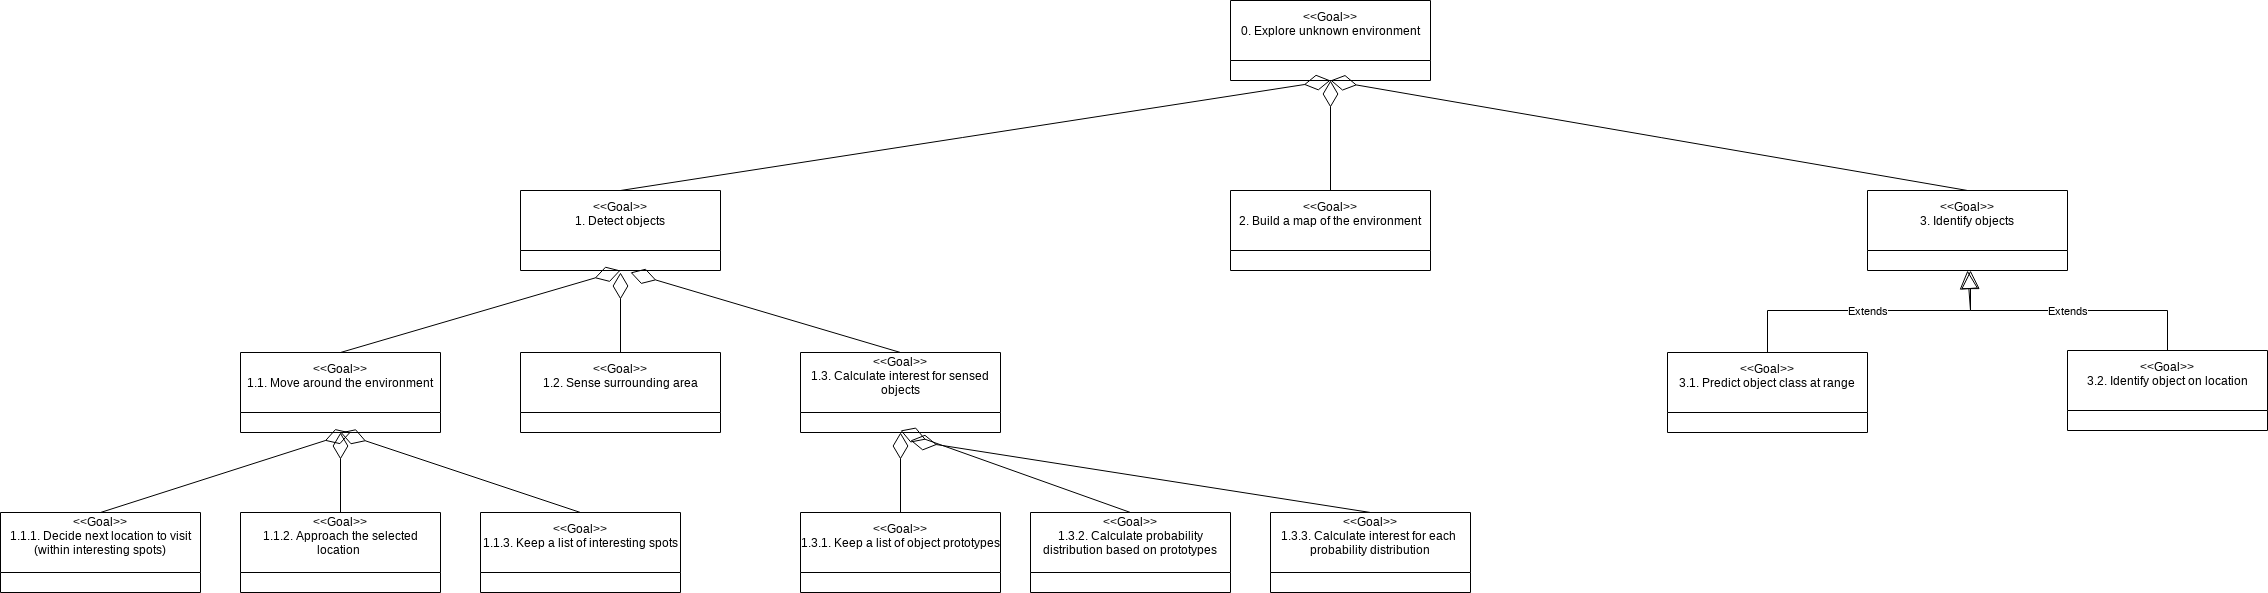
\includegraphics[width=1\linewidth]{img/goal-tree.png}
	\caption{Tree model showing the requirements (goals) of our system.}
	\label{fig:goal-tree-model}
\end{figure*}

After defining the goal tree model, we then proceed with the actual analysis phase, which starts with the creation of the organizational model shown in figure \ref{fig:organization-model}. As it is possible to evince from the model, our system has a single organization (the autonomous exploration system), which achieves the goal of exploring an unknown environment. 
\begin{figure}[htb]
	\centering
	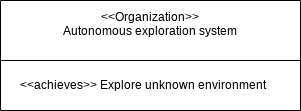
\includegraphics[width=0.5\linewidth]{img/organization-model.png}
	\caption{The organization model of our system.}
	\label{fig:organization-model}
\end{figure}

We refine the organization model into the role model shown in figure \ref{fig:role-model}. The main roles of our system are the \emph{Broker}, who decides the next position to visit for each agent, the \emph{Mapper}, who has the task to build a consistent map of the environment and store a list of objects prototype and the \emph{Explorer}, who moves around the environment, collects data and classifies objects. All these roles and the actors who play them are presented more in detail in section \ref{sec:agents-architecture}.
\begin{figure}[htb]
	\centering
	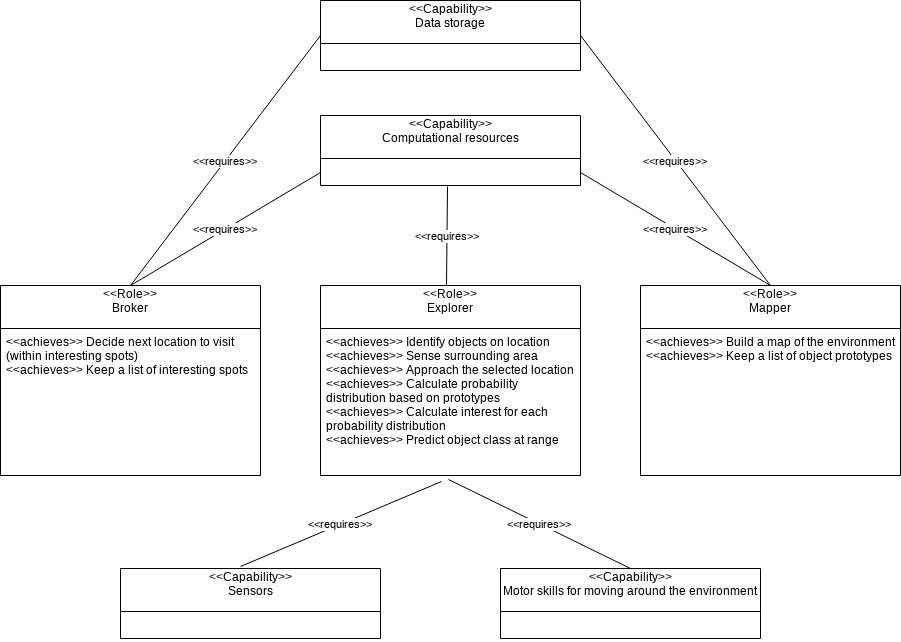
\includegraphics[width=1\linewidth]{img/role-model.png}
	\caption{The role model of our system that defines the roles in the organization, the services they provide and the capabilities required to play them.}
	\label{fig:role-model}
\end{figure}

After defining the role model, we proceed to the high-level design phase by using it for defining the agent class model shown in figure \ref{fig:agent-class-model}. From this model, it is possible to infer that in our Multi Agent system only one type of agent is present: the Explorer Agent. The agents belonging to this class play all the roles defined in the role model of figure \ref{fig:role-model} and provide the achievement of the three main sub-goals shown in the goal tree model of figure \ref{fig:goal-tree-model}. Having just one single class of agents is a consequence of the decision to adopt a peer-to-peer architecture in which there is no any central entity and every agent has the same features and provides the same services. 
\begin{figure}[htb]
	\centering
	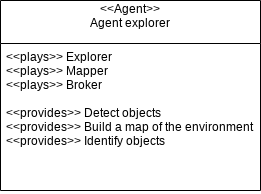
\includegraphics[width=0.5\linewidth]{img/agent-class.png}
	\caption{The agent class model of our system.}
	\label{fig:agent-class-model}
\end{figure}







\section{Methodology}
After designing and analyzing our multi agent system through the o-MaSE methodology, we proceed to the implementation of it. In this section we present all the the implementation details, from the system architecture to the algorithms and statistical formulas at the base of it. 

\subsection{System architecture}
The system architecture is composed of three main entities: the environment, the objects that populates it and a network connecting all the agents.  

The environment is a two-dimensional grid in which each cell can be populated by zero objects, one single object, one object and one agent or one single agent. Through an auxiliary two-dimensional array that contains the positions of all the agents and of the objects seen so far, every cell is considered by the agents as explored or unexplored. The positions of the objects contained in the environment are identified by the array indexes of the grid cell in which the objects are contained. 

The objects populates the environment and are characterized by a set of attributes. For simplicity, in our work we considered as attributes only the size and the colour of the object. Each object also belongs to a certain class, which correspond to a family of object of the same type with similar (but different) attributes. The classes we considered in our work are Tree, Bush, Water, House and Wall: all the objects belonging to one of these classes have similar features that make it possible to determine which class they belong to, but, individually, they are characterized by slightly different attributes. All the attributes characterizing the objects can be sensed by the agents at distance. 

The network is the means of communication that interconnect all the agents. Through the network, the agents can communicate to each other and share the knowledge they individually acquire. We implemented the network as a mere broadcasting system: when an agent sends a message to the network, that message is received by all the other agents. 

When it comes to a practical implementation of our system, some secondary aspects has to be considered. Indeed, we assumed that each agent, in every moment of the exploration, knows its exact position within the environment and communicates it to the other agents. This, in a real-life scenario, could be easily achieved by providing the agents with a GPS module. The agents in this scenario should be as well provided with a set of sensors that enable them to gather information about their surrounding area and, in particular, about the attributes of the objects they have to discover and classify. If the attributes, like in our case, are just the colour and the size, then a mere vision-enabled sensor could fit the purpose. Another consideration regarding the network interconnecting the agents has also to be done. The network, in fact, represents a core element of our system since the communication between the different agents is the only way for achieving co-operation and explore the environment in the shortest time possible. For this reason, a particular attention to this element should be given when actually implementing the system, taking thus care to use a high-performance (due to the high number of messages exchanged between the agents) and fault-tolerant network for allowing scalability and prevent the system from stopping working. 

\subsection{Agents architecture}\label{sec:agents-architecture}
As already mentioned in the introduction section, we chose to adopt a peer-to-peer architecture. For this reason, all the roles defined in the role model resulted from the agent software engineering process are played by a single actor, to which, for simplicity, from now on we will refer to as the \emph{Explorer}. Each explorer has the same features, provides the same services and co-operate with all the other explorers (its peers) for exploring the unknown environment. In particular, in relation to the role model shown in figure \ref{fig:role-model}, each explorer plays the defined roles as follows: 
\subsubsection{Mapper} in relation to this role, each explorer stores two different bi-dimensional grids: 
\begin{itemize}
    \item a grid corresponding to the current environment map in which it stores the positions of every explorer, the objects seen so far and their position. This grid basically corresponds to the current knowledge of the environment of the explorer, thus we will refer to is as the \emph{Known World}.
    \item an auxiliary grid that is used to determine whether an object in a certain position has already been identified. The grid simply stores the classes of the identified objects, using as array indexes the ones corresponding to the objects positions: if a cell is null, then it means that a possible object in that positions hasn't been identified yet. 
    \item a list of prototypes, which are abstract representations of the different objects the explorer has seen so far. Each prototype contains information about average characteristics of the associated object family and it is used by the explorer when it has to assign to a probability distribution to a new discovered object. This aspect is analyzed more in deep in the sections \ref{sec:object-classification} and \ref{sec:interest-calculation}. 
\end{itemize}

In order to build a consistent map and contribute to the object classification process, each explorer, using the network, broadcasts to its peers every new information it gets, be it its current positions, a new object prototype or the position of an object it discovered. For this reason, in order to provide to an entity external to the system (like for instance a human operator) a full view of the environment explored so far, we believe that an algorithm for merging the single maps of each explorer is not strictly necessary. Indeed, by making each explorer broadcast every new information as soon as it acquires it, the inconsistencies of the different explorers maps are negligible, since they are due only to the (supposedly low) network latency. %, thus a merging algorithm would represent an extra-overhead not worth to be introduced.  


\subsubsection{Explorer}
playing this role, the agents have the task of travelling around the environment, sense the possible objects and gain knowledge about them. For performing these tasks, the explorer has to be equipped with sensors that allow it to have a view range in all the directions and detect the attributes of the objects. It of course also must have some moving capabilities that allow him to travel around the environment at a certain speed. In our simulation environment, at each simulation step the explorer move torwards its target and senses the surrounding area included in its view range, changing its position by a number of cells proportional to its moving speed.

Whenever an object falls into the explorer view, the explorer senses its attributes, assigns it a probability distribution and, based on that distribution, calculates an interest level for that object. If the interest level is above a certain threshold, then the explorer marks that object as a possible future target since it considers worth visiting its location for identifying it and gaining more knowledge about it. If instead the interest level is below the threshold, then the explorer identifies it at distance using the probability distribution it previously computed. In the first case, when the explorer reaches the object location it has to spend some time (simulation steps) for identifying it, simulating a real-life identification scenario. When it finishes the identification, the explorer is sure about the classification result, namely the class which the object belongs to, therefore it adds the object description to the prototypes list of the identified class and broadcasts this information to the other explorers. 

\subsubsection{Broker}
according to this role, once an agent has reached its target, it has to determine which will be its next target location. For doing this, each agent stores a list of interesting locations, namely a list of unexplored locations containing objects previously sensed by the agent and for which it computed an interest level above a certain threshold. This list can be seen as the possible next targets list. When the agent has to decide its next targets, it picks from the list the location with the highest interest and it computes its distance from that location. In this way, besides the interest level, the agents also consider the distance from the possible next target, considering therefore more relevant the locations close to him that take less time to be reached. 

After choosing the highest interest location and computing the respective distance, the agent removes that location from its interesting locations list and starts an auction for determining whether that location will actually be its next target. The agent therefore broadcast to all its other peers the location and the respective interest and distance, starting in this way the bidding process for that location, that is explained more in detail in section \ref{sec:bidding-algorithm}. The agent will get that specific location as next target only if it will not receive, in a certain amount of time, any other bid from any other peer which has an higher relevance level (namely a shorter distance) for that location. 




\subsection{Objects classification}\label{sec:object-classification}
When an explorer finds a new object, it tries to classify it by assigning to it a probability distribution based on the knowledge of the environment that it has acquired so far, namely the Prototypes that him and all of its peer has developed so far. The explorer therefore goes through the list of available prototypes and correlates the attribute of each of them to the attributes of the object. This correlation consists in a weighted average of the euclidean distances between each attribute of each prototype and the object, and it represents the probability for the object to be an instance of each of the prototypes. 

The output of the correlation process described above is then multiplied by a saturation coefficient that takes into account the number of times that the explorers have seen and classified on location the objects associated to each prototype. In this way, the probability distribution considers that only after several classification of a certain type of object some knowledge about it and the corresponding prototype can be gained. Without this factor, a single object identification would be considered enough by the agents for assuming that they posses all the knowledge about that kind of object. The saturation coefficient formula is shown in equation \eqref{eq:saturation-coeff}.
\begin{equation}\label{eq:saturation-coeff}
    saturation_{coeff} = tanh(\frac{n_{occurrs}-5}{2.0}+1.0)/2.0
\end{equation}
The formula saturates close to $1.0$ when the number of occurrences ($n_{occurrs}$) of the respective object approaches ten: this means that the explorers have to identify on location at least ten objects of a certain class before assuming that they have real knowledge about that class. Summarizing, the saturation coefficient allows to weight the probability distribution according to the number of witnessed objects for each prototype. 

The explorers also have to take into account that it can happen that an object they witnessed does not belong to any of the defined prototypes. This is done by calculating the \emph{unknown correlation}, namely a value that estimates the probability that the found object does not belong to any prototype. When the number of available prototype is equal or greater than one, this correlation is calculated using the formula shown in equation \eqref{eq:unknown-correlation}, otherwise it is automatically set to $1$ when no prototypes are available. 
\begin{equation}\label{eq:unknown-correlation}
    unknown_{corr} = \sum_{i=1}^{N} \frac{1-corr(i)}{N}
\end{equation}
In equation \eqref{eq:unknown-correlation}, $N$ represents the total number of available prototypes while $corr(i)$ corresponds to the correlation (saturation coefficient included) of the object to the $i^{th}$ prototype. The unknown correlation is maximum when all the correlations are equal to $0$ (it means that the object actually represents ``something new'') and it is minimum when all the correlations are $1$ (it means that the object fits all the prototypes). 

Considering the correlations calculation process described above, the explorers finally compute the probability distribution by transforming the calculated correlations according to equation \eqref{eq:probability-distribution}. The obtained probability distributions, that sums to $1$, expresses the probabilities that the object is an instance of each single prototype, and the probability that the object belong to the ``unknown''.
\begin{equation}\label{eq:probability-distribution}
    p(j) = \frac{corr(j)}{\sum_{i=1}^{N}corr(i)}
\end{equation}
In equation \eqref{eq:probability-distribution} $p(j)$ corresponds to the probability associated to the prototype $j$, while $N$ represents the number of available prototypes plus $1$ (the unknown). 

\subsection{Interest level calculation}\label{sec:interest-calculation}
As already mentioned, whenever an explorer witnesses an object it calculates its interest level. This interest is based on the probability distribution described in the previous section and it is calculated in two different steps. 

In the first step the explorer computes the interest level related to the probability of finding a new object that does not belong to any of the known classes, namely the \emph{unknown interest}. This is done by mapping the unknown probability $p(unknown)$ as defined in equation \eqref{eq:unknown-interest}.
\begin{equation}\label{eq:unknown-interest}
    unknown_{interest} = tanh(2.0 \times p(unknown))
\end{equation}
The formula shown in equation \eqref{eq:unknown-interest} merely increases the rate of climb of the interest respectively to the increase of the unknown probability. Indeed, without it, if the unknown probability was 50\% then the interest level would be 50\% as well: we want to avoid this since we consider that an unknown probability of 50\% should correspond to an higher interest level. 

Besides considering interesting the unknown, the explorer also considers interesting objects that have similar characteristics to several known classes. For this reason, the explorer computes another interest level, the \emph{chaotic interest}, as defined in equation \eqref{eq:chaotic-interest}. 
\begin{equation}\label{eq:chaotic-interest}
    chaotic_{interest} = - \sum_{i=1}^{N}p(i)\times log(p(i))
\end{equation}
The equation \eqref{eq:chaotic-interest} basically corresponds to the entropy of the probability distribution: high entropy values represent more chaotic situations, that the agents consider interesting. 

After calculating the \emph{unknown interest} and the \emph{chaotic interest}, the explorer chooses as interest value the highest one between these two and assigns it to the object in question. Once the interest level has been assigned to the object, the explorer decides whether that object has an high enough interest to be visited on location, or whether the object is not interesting enough to be visited. In the first case the object location is added to the interesting locations list, namely the list containing the next potential targets of the explorer, while in the latter case the explorer classifies the object at range as described in section \ref{sec:object-classification}. In this latter case, after the explorer classifies the object, it broadcasts the information to all its peers so that they can update their map according to the new knowledge they have acquired. 

The \emph{interest threshold} is the parameter that determines which objects the explorer considers interesting enough: if the interest level is above this threshold, then the explorer adds the respective object to the next potential target list, otherwise it classifies it at distance. 




\subsection{The Bidding algorithm}\label{sec:bidding-algorithm}
After an explorer reaches its target, it has to determine which its next target location will be. In order to do so, it communicates to its peers and runs a distributed algorithm, e.g. the \emph{bidding algorithm}, that allows him (and its peers) to get as target the best possible location between all the unexplored ones. This algorithm can be seen as an \emph{auction} to which participate all those explorers that have already reached their target and are waiting for a new one, and which is carried out through a series of \emph{bids} made by these agents.  

When an explorer reaches its target, it picks from its (personal) list of possible next target the location containing the object with the highest interest level. Then, the explorer computes its distance from that location and starts the auction for the respective location by sending to all of its peers a bid. The bid is nothing more then a tuple composed of the object location (e.g. the next potential target), the interest level and the distance of that location from the explorer that sends the bid. After sending the bid, the agent waits a certain amount of time (we will refer to it as \emph{TIME\_WAIT\_BID\_REPLY}): if, when this amount of time has elapsed, the agent has not received any other bid for that location by the other explorers, then he can consider himself as the winner of the auction and its next target becomes the location in question. 
When an explorer that is waiting for its next target receives a bid for a certain location by some other explorer, it computes its distance from that location. If its distance is lower than the distance value included in the bid it received, namely the distance of the location from the explorer who made the bid, it means that the location is more relevant for him and therefore it checks whether it is worth to participate to the auction for that location by replying with another bid. Consequently, if the explorer was already participating to another auction, it checks whether its distance from the location associated to the auction he was participating is higher than its distance from the new location it received within the bid: in this case, it gives up with the previous auction and it replies with a new bid to the auction for the other location, because it means that the new location included in the bid it received is more relevant for him. After replying, the explorer has to wait again TIME\_WAIT\_BID\_REPLY before considering himself as the winner and start moving towards the new acquired target.

Thanks to this algorithm, we assure not only that the most interesting locations are visited first, but also that these locations are visited by the explorers which are the closest to them, limiting consequently the time that the explorers spend travelling around the environment for reaching their targets. 

It is important to point out two details concerning this algorithm:
\begin{itemize}
    \item whenever an explorer makes a bid for a certain location, it removes that location from its interesting locations list and it broadcasts this information to all its peers: all the explorers which also have that location within their list (e.g. they also previously witnessed the object in that location and add it to their interesting locations list) then proceed to remove it as well. In this way, we avoid that more auctions are made for the same location, since this behaviour would represent a waste of time and resources. 
    \item when an explorer is participating to an auction for a certain location and it gives up for participating to another auction related to another location for which he has higher relevance (shorter distance), the previous location associated to the auction he quit is added again to his personal list of interesting locations. This is done in order to avoid that, in the case the explorer who quit was supposed to be the winner of that auction, the location, besides not being the target of any explorer, is also be excluded from all the future auctions. In this way instead, the location can be part of another future auction since the explorer who previously discarded it will pick it up later from his interesting locations list.
\end{itemize}


\section{Experimental setup}
In order to measure the performance of our system, we tested groups of agents with multiple different configurations. In particular, since our system is basically a peer-to-peer adaptation of the system implemented in \cite{tavaresgaspar}, we also adopted a set of similar configurations in order to fairly compare the performance of our approach with the one of the master-slave architecture used in the mentioned work. 

Table \ref{tab:configurations} summarizes all the configurations we adopted.
\begin{table*}[htb]
    \centering
    \begin{tabular}{|c|c|c|c|c|c|c|}
        \hline
         Config. & Environment & N agents & Interest threshold & View radius & TIME\_WAIT\_BID\_REPLY \\  \hline  
         1 & Structured & 10 & 40 & 40 & 15 \\
         2 & Structured & 10 & 50 & 40 & 15 \\
         3 & Structured & 10 & 65 & 40 & 15 \\
         4 & Structured & 10 & 75 & 40 & 15 \\
         5 & Structured & 10 & 90 & 40 & 15 \\
         6 & Structured & 10 & 65 & 20 & 15 \\
         7 & Structured & 10 & 65 & 60 & 15 \\
         8 & Structured & 10 & 65 & 40 & 5 \\
         9 & Structured & 10 & 65 & 40 & 25 \\
         10 & Structured & 2 & 65 & 40 & 15 \\
         11 & Structured & 5 & 65 & 40 & 15 \\
         12 & Structured & 10 & 65 & 40 & 15 \\
         13 & Structured & 20 & 65 & 40 & 15 \\ \hline
    \end{tabular}
    \caption{The different configurations we used to perform our tests}
    \label{tab:configurations}
\end{table*}

The environment we used to test the capabilities of our system is the Structured Environment, presented in \cite{tavaresgaspar} and shown in figure \ref{fig:structured-environment}. This environment represents a pseudo-real exploration scenario (it could for instance represent a neighborhood) and it is populated with 5 different types of objects: bushes, houses, trees, walls and water. The total number of objects is around 3500, a number high enough for representing the kind of situation in which a multi-agent system with partially predictive mapping like the one we implemented can (theoretically) clearly show how its performance is better than a classic approach. In this environment moreover, some classes of objects may be very similar to one another (such as bushes and trees). This aspect enables us to test the accuracy of object classification with objects that are similar but not the same and, as such, should be classified as different objects.

In the different configurations we used we varied the number of agents, the threshold over which an agent finds a certain object interesting, the view radius of the agents and the value of TIME\_WAIT\_BID\_REPLY. Besides the simulation environment, some other simulation parameters are fixed in all the configurations and shared with the work in \cite{tavaresgaspar}, such as the simulation time and the time required to identify an object, which are, respectively, 5000 and 15 steps.


\section{Results}\label{sec:resuslts}

\begin{figure}[h]
	\centering
	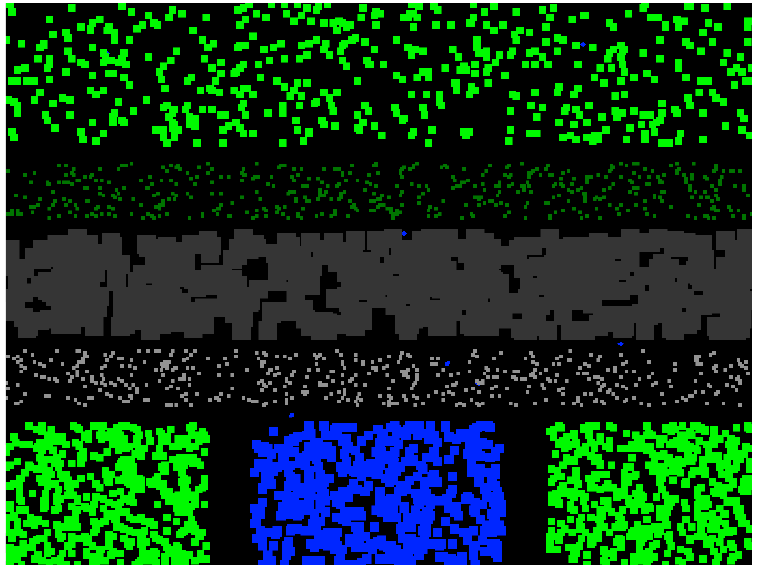
\includegraphics[width=1\linewidth]{img/structured-environment.png}
	\caption{The structured environment}
	\label{fig:structured-environment}
\end{figure}

In this section we present and discuss the results we obtained from our tests. The results are shown for all the different configurations we used and they are presented in graphical form through charts that, for each single simulation step, show the percentages of explored environment and committed error up to that specific step. In order to provide a more accurate estimation of the performance of our system, all the results presented in this section have been collected by running the simulation 50 times for each configuration and doing an average of the obtained values. For each of these 50 simulations, we decided to set the starting position of the explorers randomly.

The results are organized in five different sections. The first four sections group different configurations together according to the parameters that we varied for that set of tests. The fourth section is dedicated to present the results in term of number of messages exchanged between the agents. Finally, we decided to dedicate the last section to a brief comparison between the performance of our system and the one described in \cite{tavaresgaspar}, in which a master-slave approach is used instead of peer-to-peer one. Given the similarity of the two works, we believe that a performance comparison can be carried our in a fair way and it can be useful for later exploring better the advantages and disadvantages of each of the two approaches. 



\subsection{Changing Interest Threshold}
Here are presented the results of the configurations in which we varied the interest threshold value (namely configurations 1, configuration 2, configuration 3 and configuration 4, according to table \ref{tab:configurations}), keeping fixed the rest of the parameters. 
\begin{figure}[H]
	\centering
	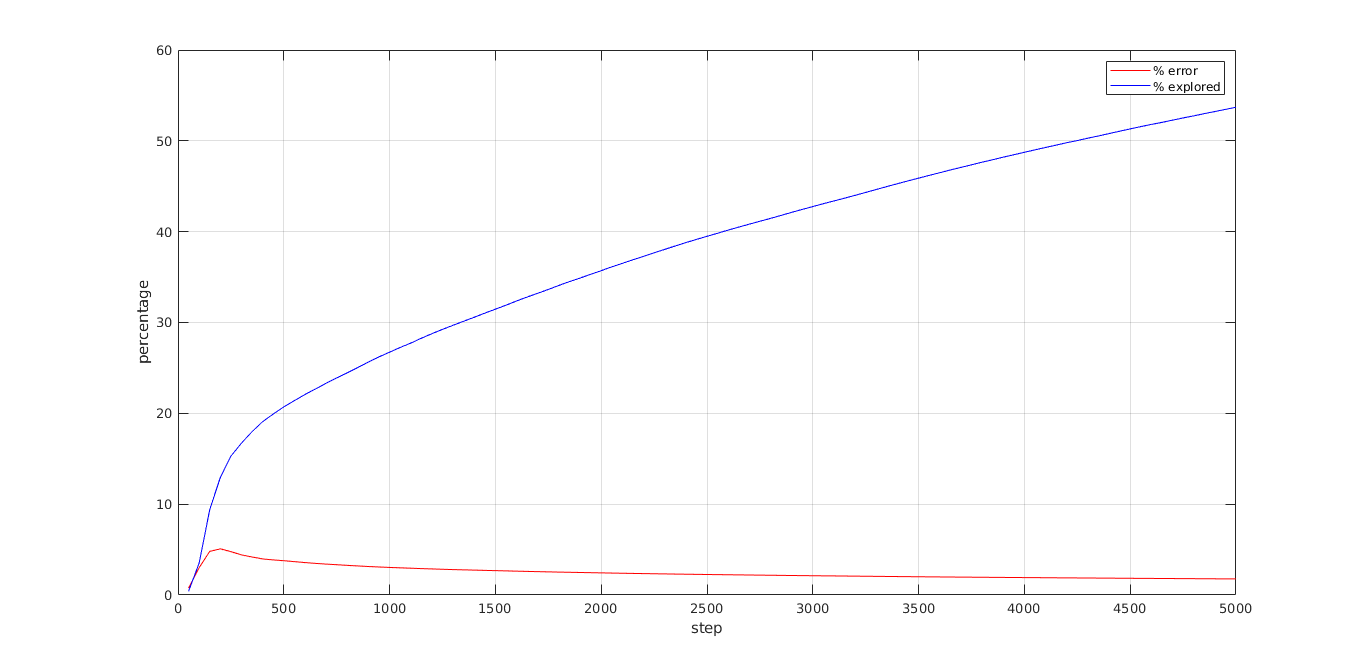
\includegraphics[width=1\linewidth]{img/config1.png}
	\caption{Configuration 1: 10 agents, Threshold=40, View radius=40, TIME\_WAIT\_BID\_REPLY=15}
	\label{fig:config1}
\end{figure}
\begin{figure}[H]
	\centering
	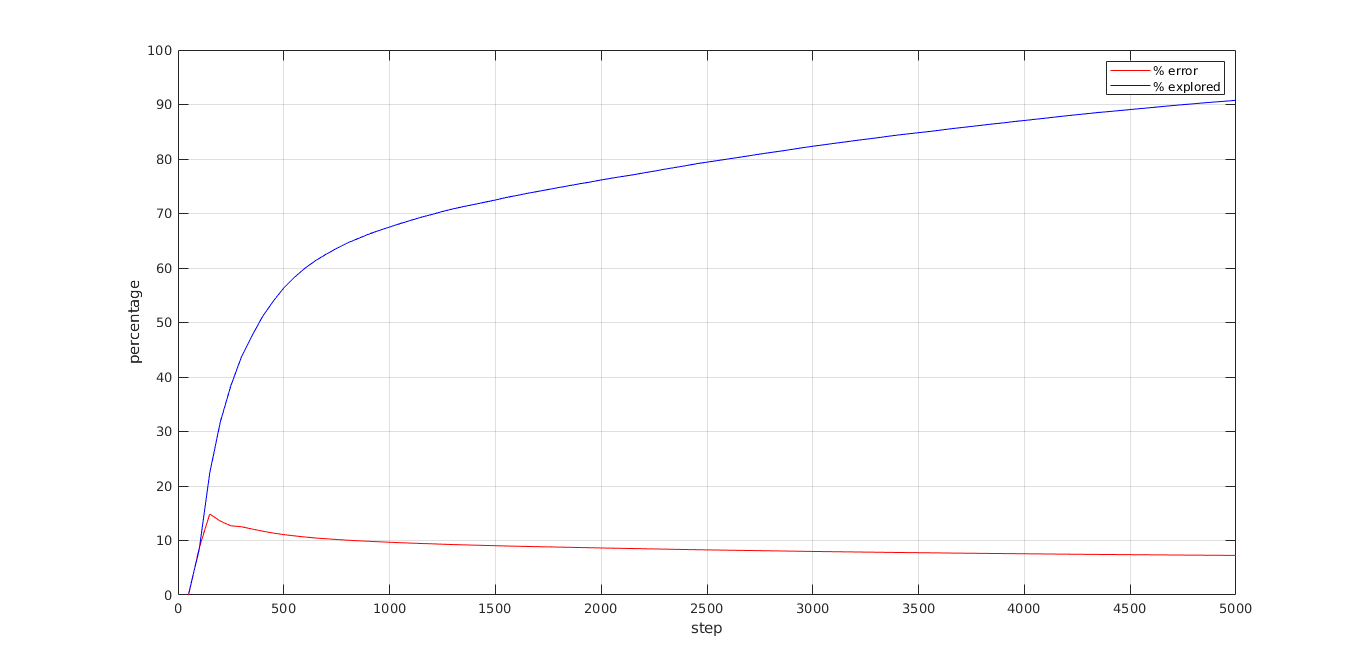
\includegraphics[width=1\linewidth]{img/config2.png}
	\caption{Configuration 2: 10 agents, Threshold=50, View radius=40, TIME\_WAIT\_BID\_REPLY=15}
	\label{fig:config2}
\end{figure}
\begin{figure}[H]
	\centering
	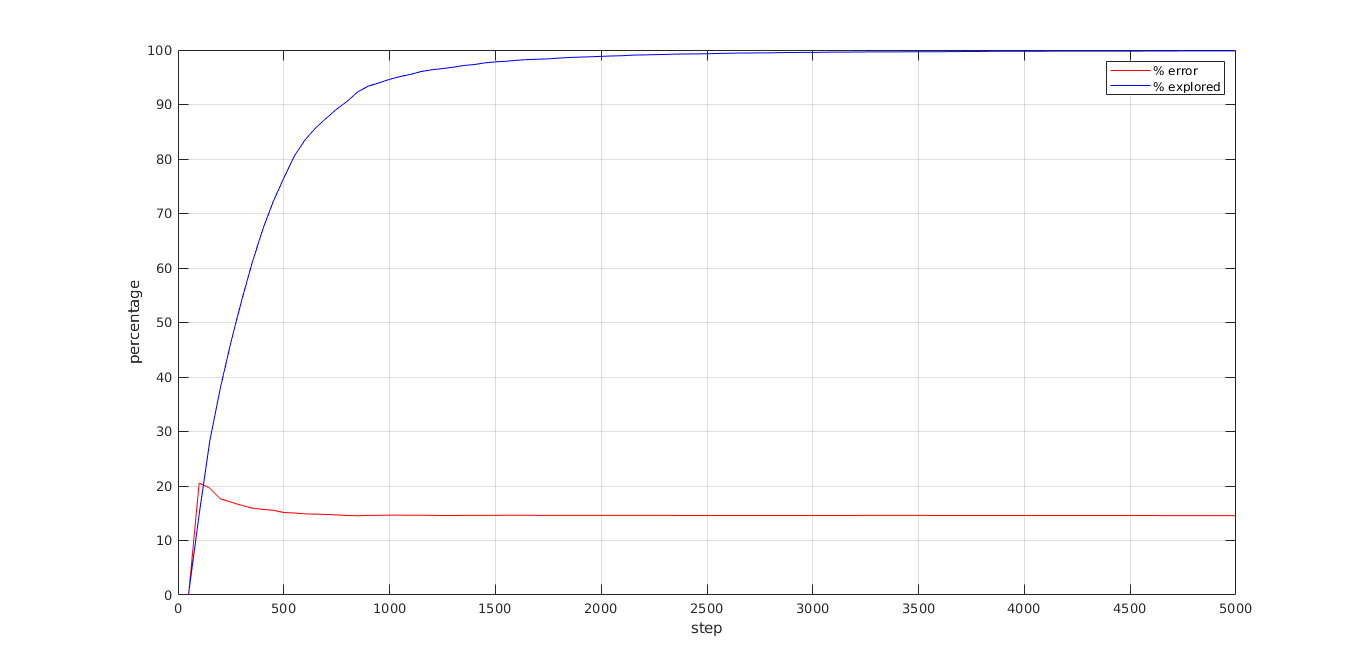
\includegraphics[width=1\linewidth]{img/config3.png}
	\caption{Configuration 3: 10 agents, Threshold=65, View radius=40, TIME\_WAIT\_BID\_REPLY=15}
	\label{fig:config3}
\end{figure}
\begin{figure}[H]
	\centering
	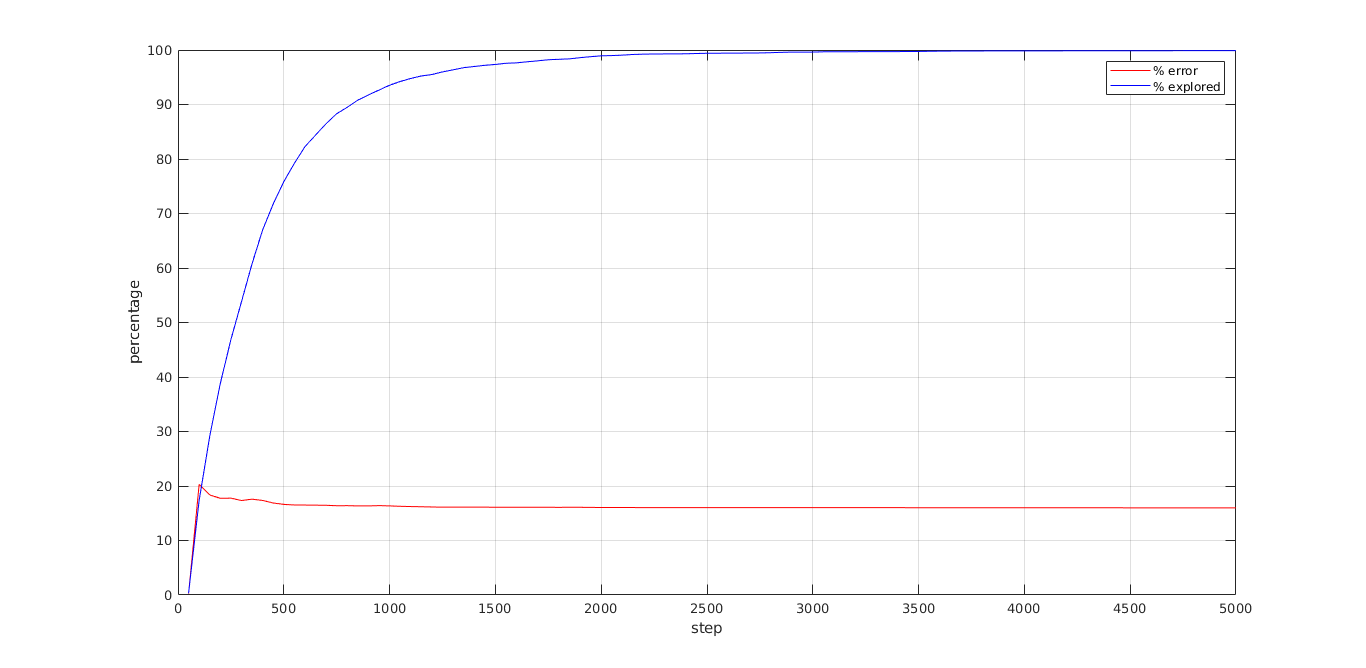
\includegraphics[width=1\linewidth]{img/config4.png}
	\caption{Configuration 4: 10 agents, Threshold=75, View radius=40, TIME\_WAIT\_BID\_REPLY=15}
	\label{fig:config4}
\end{figure}
\begin{figure}[H]
	\centering
	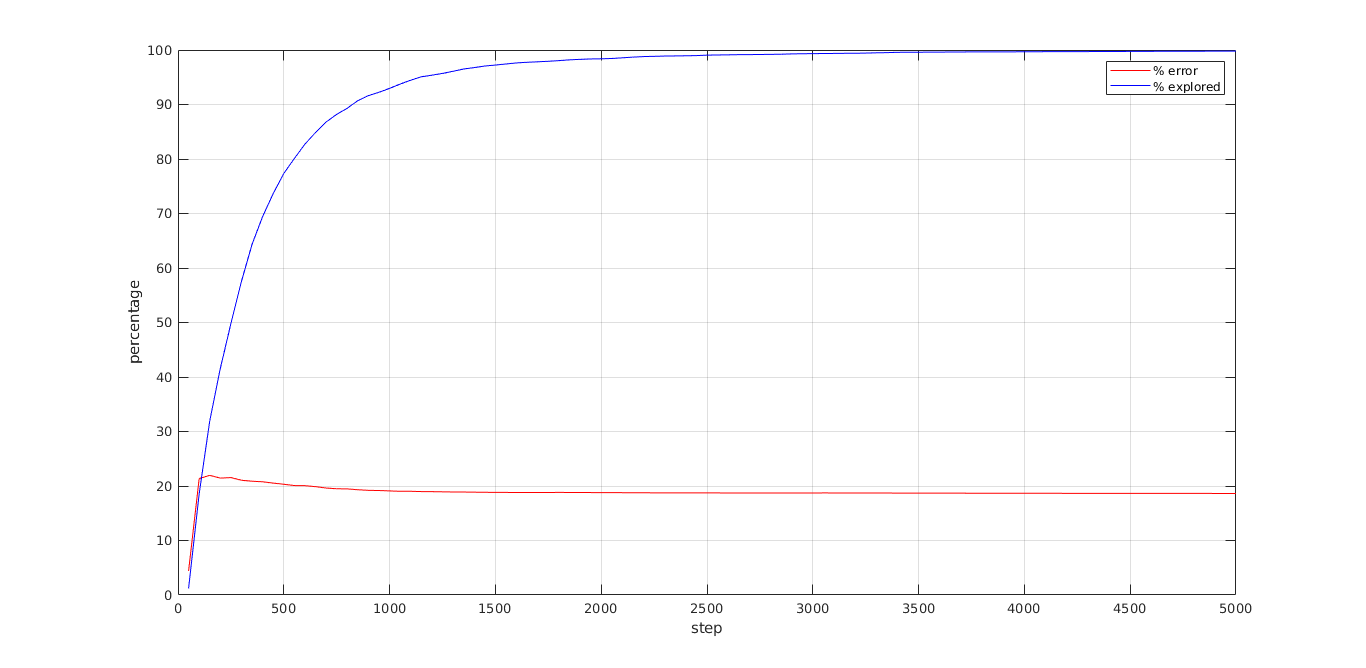
\includegraphics[width=1\linewidth]{img/config5.png}
	\caption{Configuration 5: 10 agents, Threshold=90, View radius=40, TIME\_WAIT\_BID\_REPLY=15}
	\label{fig:config5}
\end{figure}

As expected, higher values of the thresholds imply a shorter exploration time (the agents take less time to identify the objects), as well as a higher error rate. This is due to the fact that, by increasing the threshold, the agents tend to classify on location fewer objects, preferring the less time consuming classification based on the probability distribution. 

It is possible to note that with a threshold value equal to 40 the agents are able to explore not even the 60\% of the environment, even though the error they commit in classifying objects is definitely low (less than 5\%). On the other hand, by using a threshold value equal to 90 we achieve a fast exploration, with the drawback of introducing an high error in the classification process. Consequently, the threshold value must be properly balanced in order to obtain a fast enough exploration with an acceptable degree of error. We can see that a value between 65 and 75 represents a good compromise between exploration speed and error rate: for this reason, in all the other configurations that we used in our tests we decided to fix the value of the threshold parameter to 65. 



\subsection{Changing View Radius}
Here we present the results we got by varying the View Radius of the agents, keeping fixed all the other parameters (Number of Agents=10, Threshold=65, TIME\_WAIT\_BID\_REPLY=15). The configurations corresponding to this parameter variations are configuration 6, configuration 3 and configuration 7, according to table \ref{tab:configurations}.  
\begin{figure}[H]
	\centering
	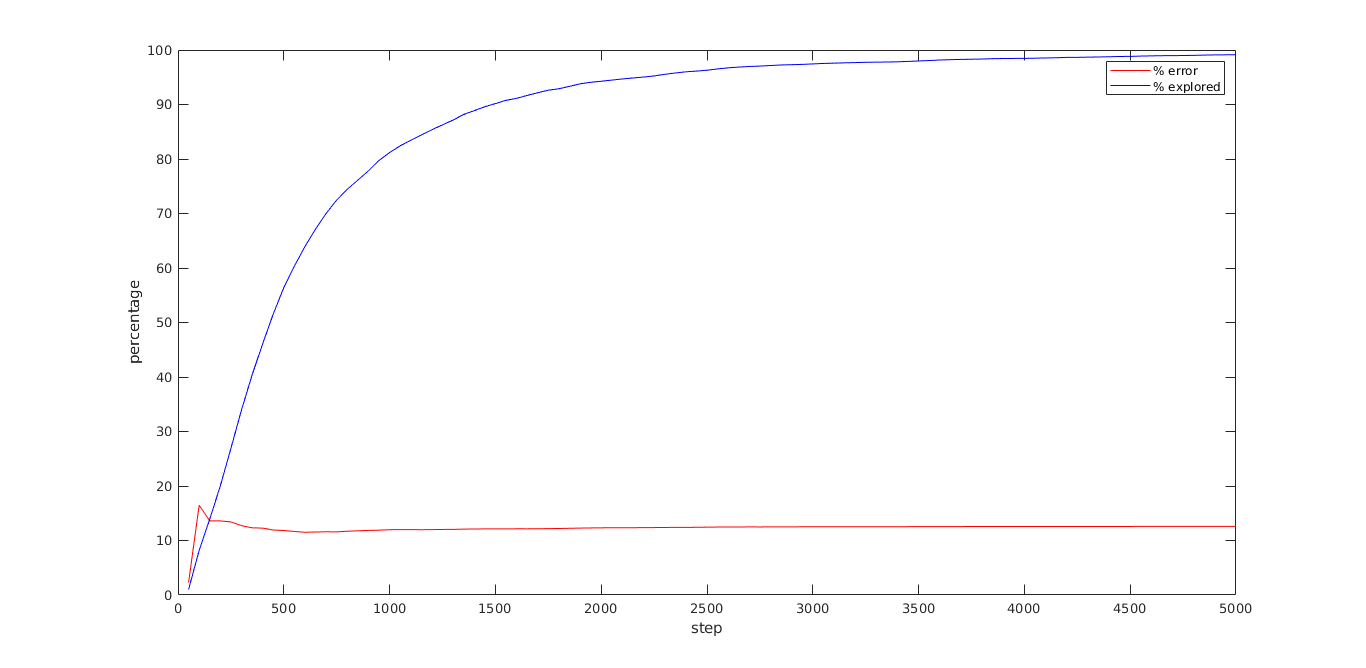
\includegraphics[width=1\linewidth]{img/config6.png}
	\caption{Configuration 6: 10 agents, Threshold=65, View radius=20, TIME\_WAIT\_BID\_REPLY=15}
	\label{fig:config6}
\end{figure}
\begin{figure}[H]
	\centering
	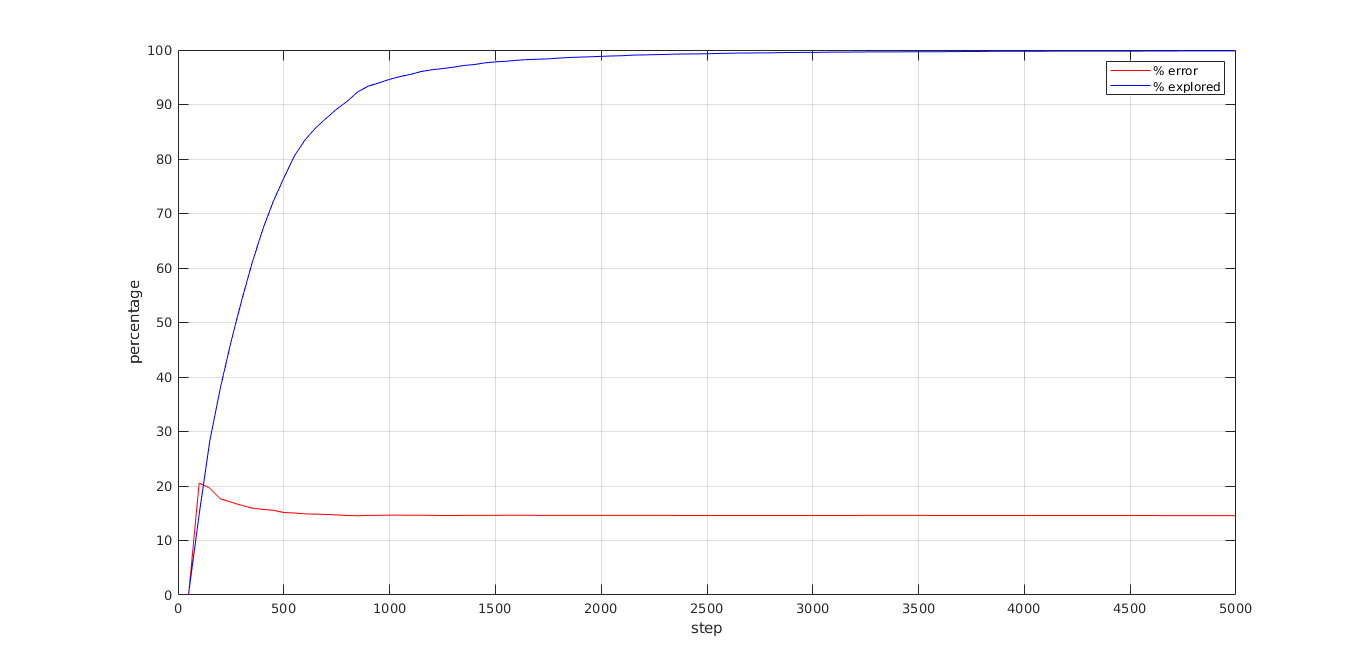
\includegraphics[width=1\linewidth]{img/config3.png}
	\caption{Configuration 3: 10 agents, Threshold=65, View radius=40, TIME\_WAIT\_BID\_REPLY=15}
	\label{fig:config3}
\end{figure}
\begin{figure}[H]
	\centering
	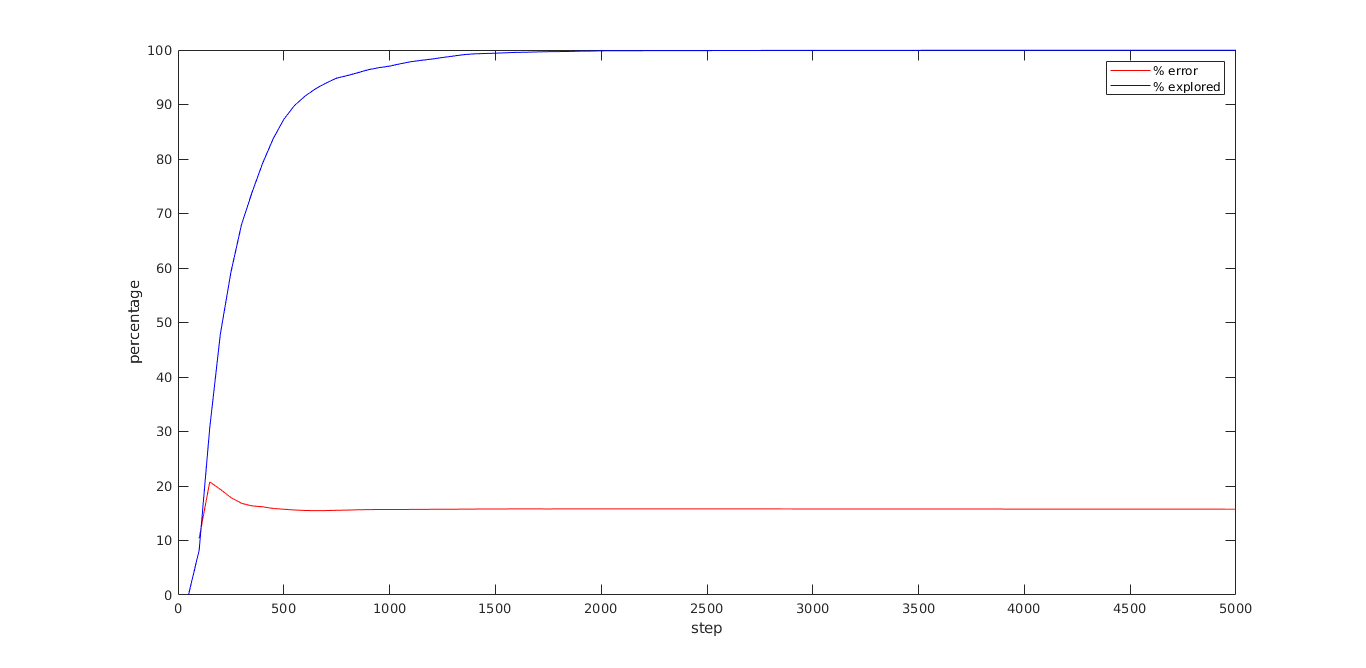
\includegraphics[width=1\linewidth]{img/config7.png}
	\caption{Configuration 7: 10 agents, Threshold=65, View radius=60, TIME\_WAIT\_BID\_REPLY=15}
	\label{fig:config7}
\end{figure}

As it was intuitively expected, the results prove that by increasing the view radius of the agents the exploration time decreases, since the agents are able to spot more objects and gain knowledge about the environment more quickly. However, together with the exploration speed, the classification error slightly increases as well. This is mainly due to the fact that by increasing the view radius the agents are able to classify more objects at distance (farther objects can be classified), increasing therefore the probability of committing errors. 

\subsection{Changing TIME\_WAIT\_BID\_REPLY}
Here we present the results we got by varying parameter TIME\_WAIT\_BID\_REPLY, keeping fixed all the other parameters (Number of Agent=10, Threshold=65, View Radius=40). The configurations corresponding to this parameter variations are configuration 8, configuration 3 and configuration 9, according to table \ref{tab:configurations}. 
\begin{figure}[H]
	\centering
	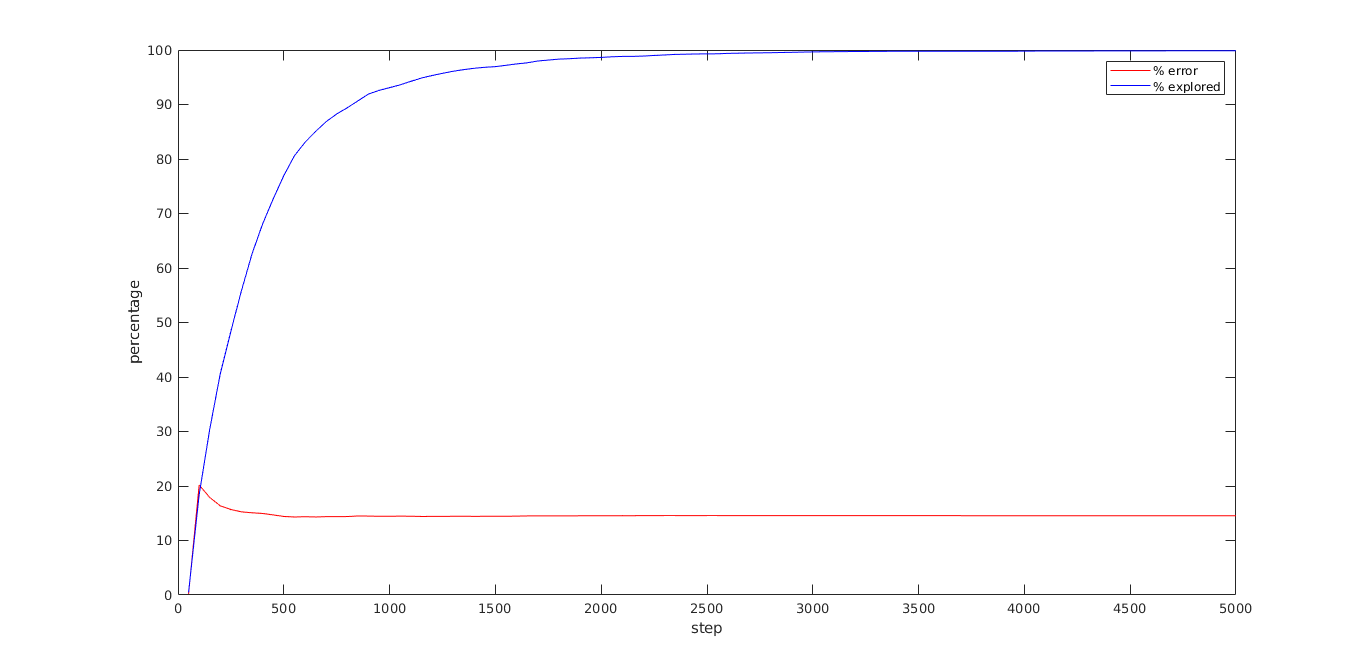
\includegraphics[width=1\linewidth]{img/config8.png}
	\caption{Configuration 8: 10 agents, Threshold=65, View radius=40, TIME\_WAIT\_BID\_REPLY=5}
	\label{fig:config8}
\end{figure}
\begin{figure}[H]
	\centering
	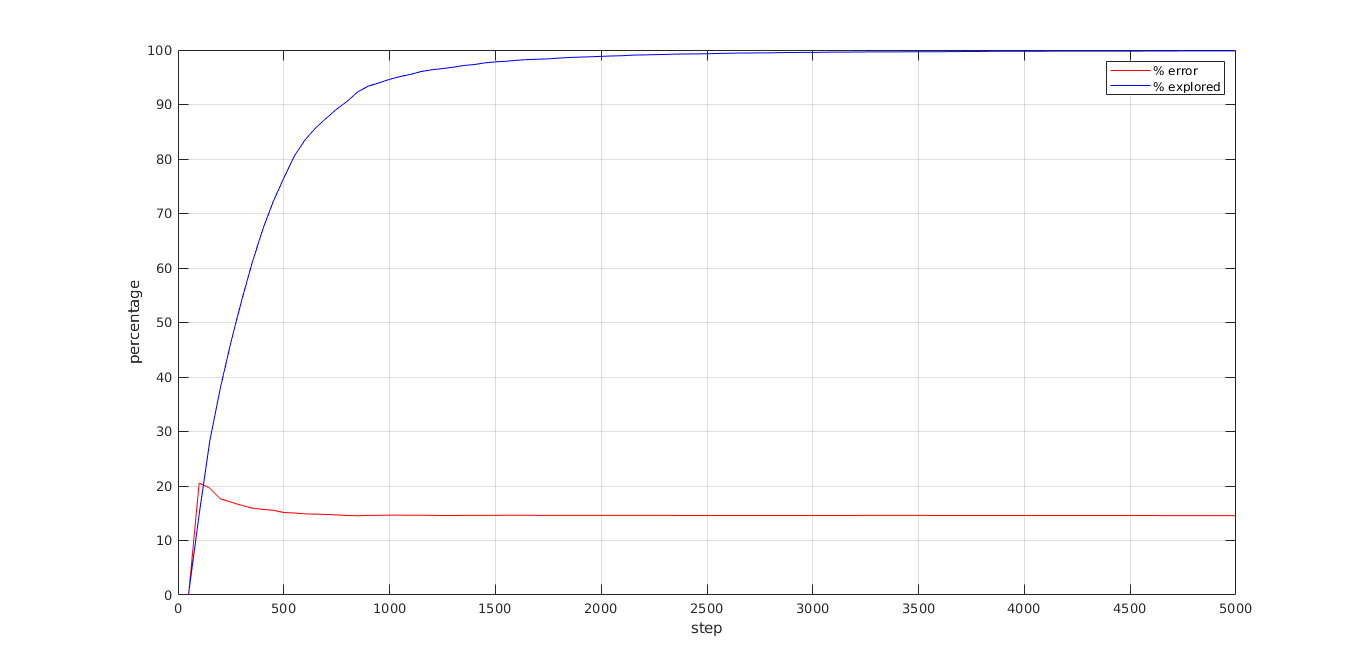
\includegraphics[width=1\linewidth]{img/config3.png}
	\caption{Configuration 3: 10 agents, Threshold=65, View radius=40, TIME\_WAIT\_BID\_REPLY=15}
	\label{fig:config3}
\end{figure}
\begin{figure}[H]
	\centering
	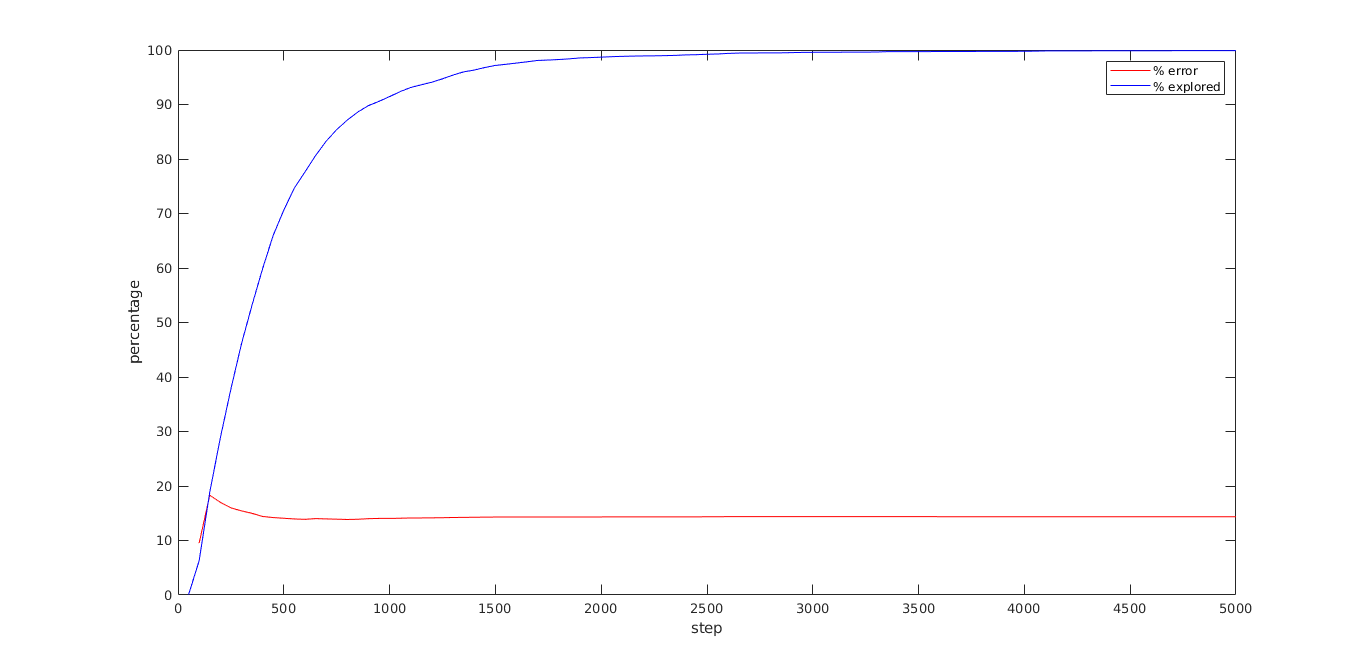
\includegraphics[width=1\linewidth]{img/config9.png}
	\caption{Configuration 9: 10 agents, Threshold=65, View radius=60, TIME\_WAIT\_BID\_REPLY=25}
	\label{fig:config9}
\end{figure}

We can notice that changing the parameter TIME\_WAIT\_BID\_REPLY, namely the time that an agent has to wait before considering himself the winner of a bid, does not affect a lot the committed classification error. Indeed, the main difference in the error rate trend that we can see from the plots in figure \ref{fig:config8}, \ref{fig:config3} and \ref{fig:config9} is that by using an high value (e.g. 25 seconds), the initial typical error peak gets more attenuated, even though the overall percentage on which the error stabilizes essentially remains the same. The exploration speed however seems to be better when using a time equal to 15 seconds: even though the time required for reaching approximately 100\% of explored environment is basically the same for all the tested values, the percentage trend is way steeper when using the mentioned value. For these reasons we believe that a TIME\_WAIT\_BID\_REPLY value equals to 15 seconds represents our best choice.

Note that 15 seconds also corresponds to the time required by the agents for classifying an object on location. Keeping in mind that agents can run the bidding algorithm even while they are classifying an object on location, using values higher than 15 seconds means that it can happen that an agent, after he finishes to classify an object, still has to wait motionless in the same position for the elapsing of TIME\_WAIT\_BID\_REPLY even if he has not received any other bid, increasing therefore the time required for exploring the whole environment. Generally, higher values of TIME\_WAIT\_BID\_REPLY imply more time spent by the agents for running the bidding algorithm (e.g. for knowing their next target), time in which they stay firm in one position without going on with the environment exploration, affecting therefore negatively the overall exploration speed. Contrarily, adopting a too small value for TIME\_WAIT\_BID\_REPLY causes an agent to consider himself as the winner of an auction ``too quickly'', reducing in this way the possibility that other agents closer to the location in question reply to the bid. This causes a decrease of efficiency in the agents coordination process, leading thus to a slower exploration of the environment.

\subsection{Changing Number of Agents}
Here are presented the results we got by varying the number of agents in the system, keeping fixed all the other parameters (Threshold=65, View Radius=40, TIME\_WAIT\_BID\_REPLY=15). The configurations corresponding to this parameter variations are configuration 10, configuration 11, configuration 12 and configuration 13, according to table \ref{tab:configurations}. 
\begin{figure}[H]
	\centering
	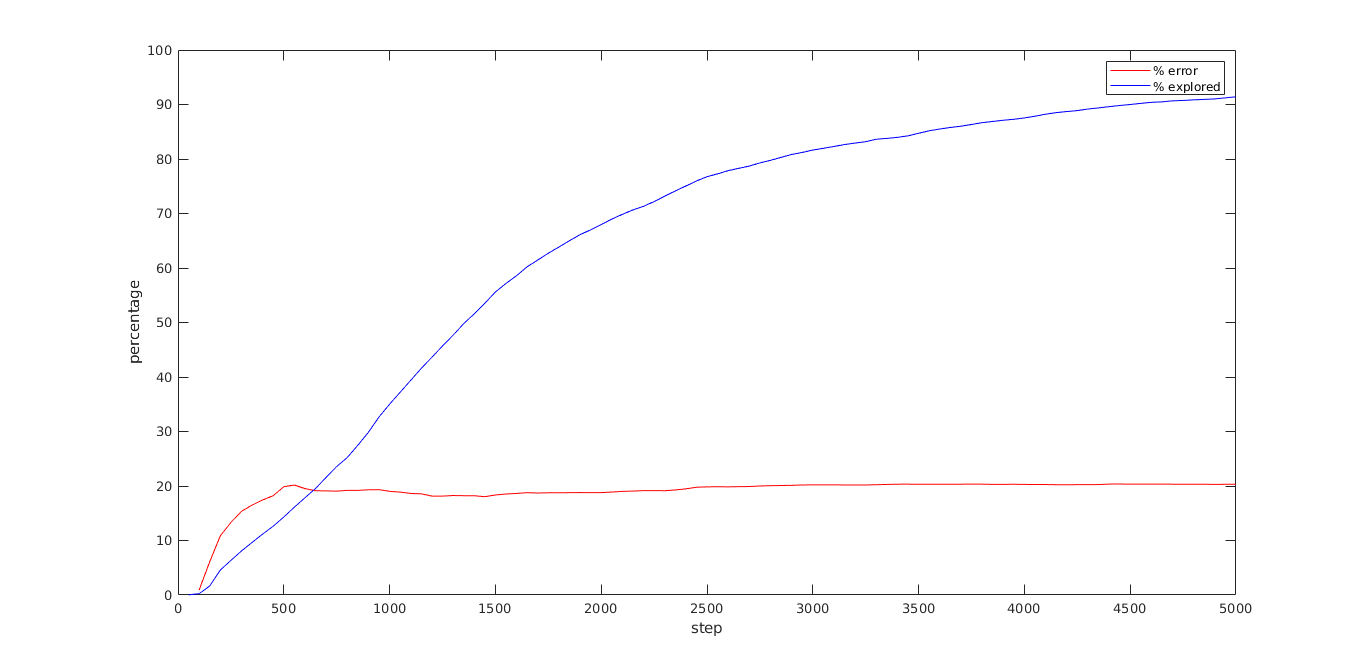
\includegraphics[width=1\linewidth]{img/config10.png}
	\caption{Configuration 10: 2 agents, Threshold=65, View radius=40, TIME\_WAIT\_BID\_REPLY=15}
	\label{fig:config10}
\end{figure}
\begin{figure}[H]
	\centering
	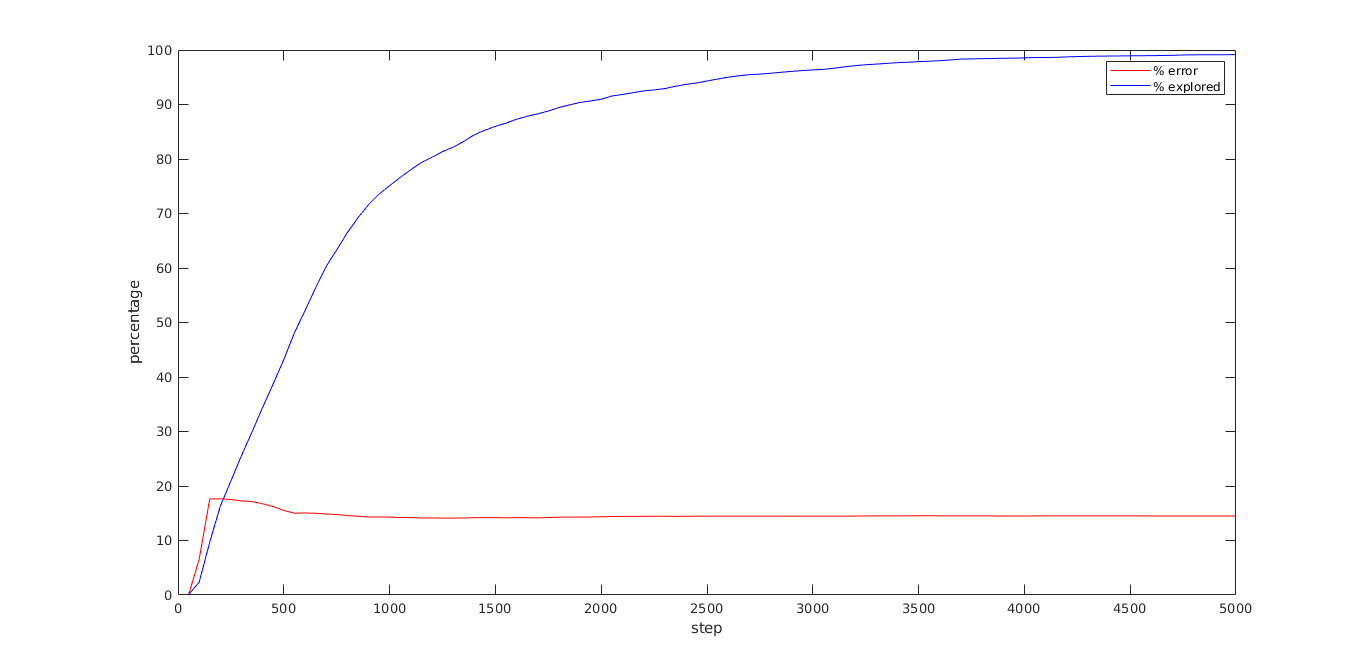
\includegraphics[width=1\linewidth]{img/config11.png}
	\caption{Configuration 11: 5 agents, Threshold=65, View radius=40, TIME\_WAIT\_BID\_REPLY=15}
	\label{fig:config11}
\end{figure}
\begin{figure}[H]
	\centering
	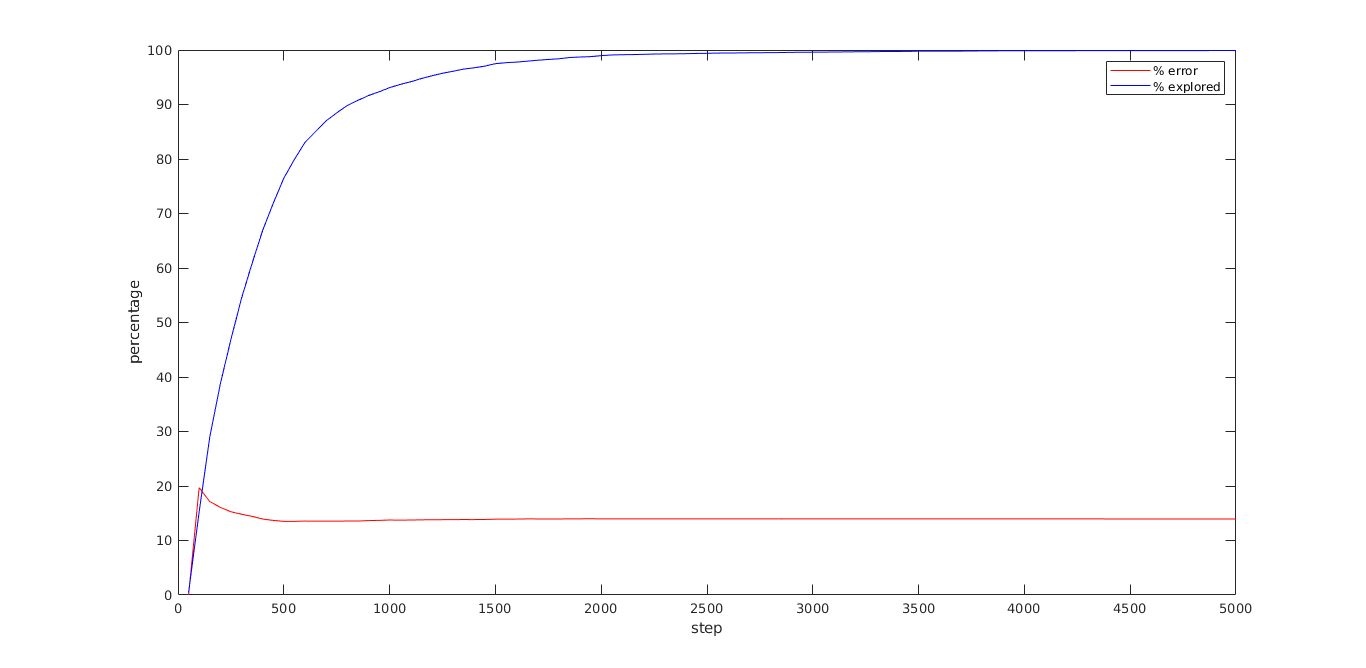
\includegraphics[width=1\linewidth]{img/config12.png}
	\caption{Configuration 10: 10 agents, Threshold=65, View radius=40, TIME\_WAIT\_BID\_REPLY=15}
	\label{fig:config12}
\end{figure}
\begin{figure}[H]
	\centering
	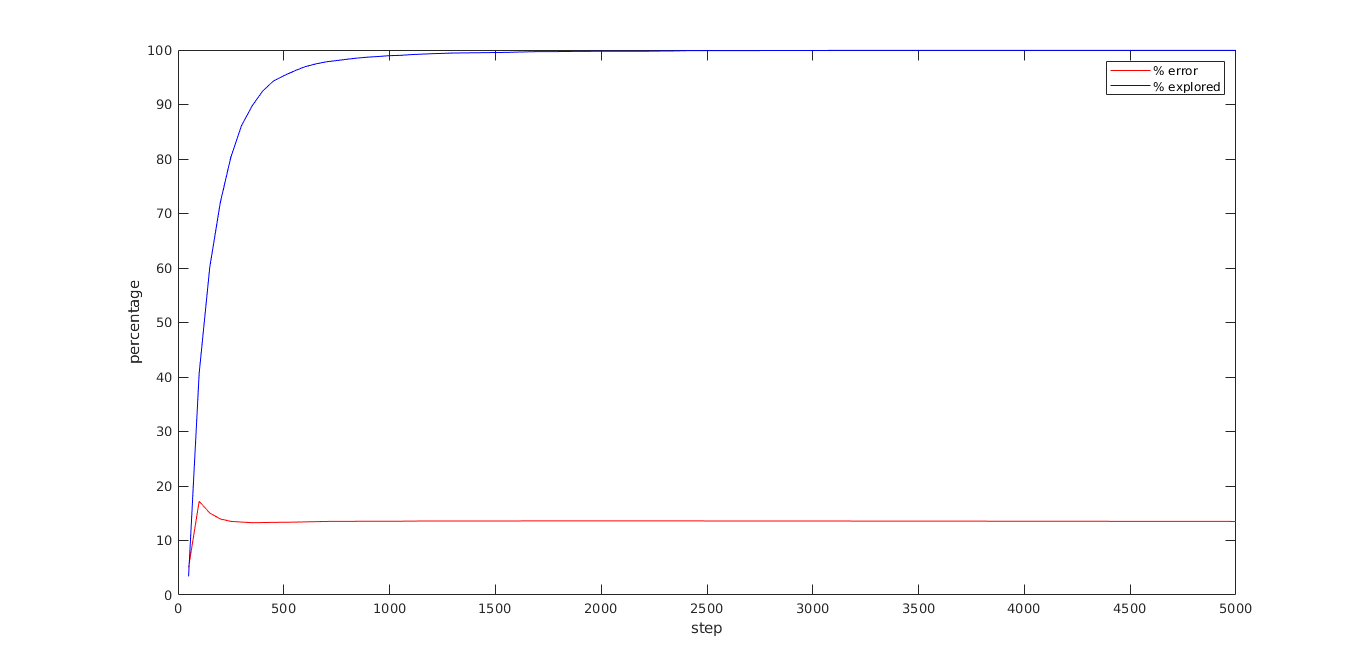
\includegraphics[width=1\linewidth]{img/config13.png}
	\caption{Configuration 13: 20 agents, Threshold=65, View radius=40, TIME\_WAIT\_BID\_REPLY=15}
	\label{fig:config13}
\end{figure}

By increasing the number of agents, the explored environment percentage trend becomes drastically steeper, while however the time required for exploring broadly 100\% of the environment still remains around 2500 steps. As expected therefore, the results prove that the performance of the system in term of exploration time improves with the number of increasing agents, showing in particular how this performance improvement mainly consists in reaching faster an explored environment percentage of 90\%. 

From the plots in figure \ref{fig:config10}, \ref{fig:config11}, \ref{fig:config12} and \ref{fig:config13}, it is also possible to notice that the classification error decreases when increasing the number of exploring agents. This is partially due to the fact that by using many agents starting in various random position of the environment, a better knowledge of the world is quickly gained by the team of agents, which is then exploited for classifying the objects more accurately, since the explorers have a more accurate shared knowledge of their surroundings. 



\subsection{Number of messages}
In this section we provide the results in term of number of messages exchanged between the agents. Specifically, we show how the number of exchanged messages varies according to the adopted threshold level, to the number of agents and to the value of TIME\_WAIT\_BID\_REPLY. 
\begin{figure}[H]
	\centering
	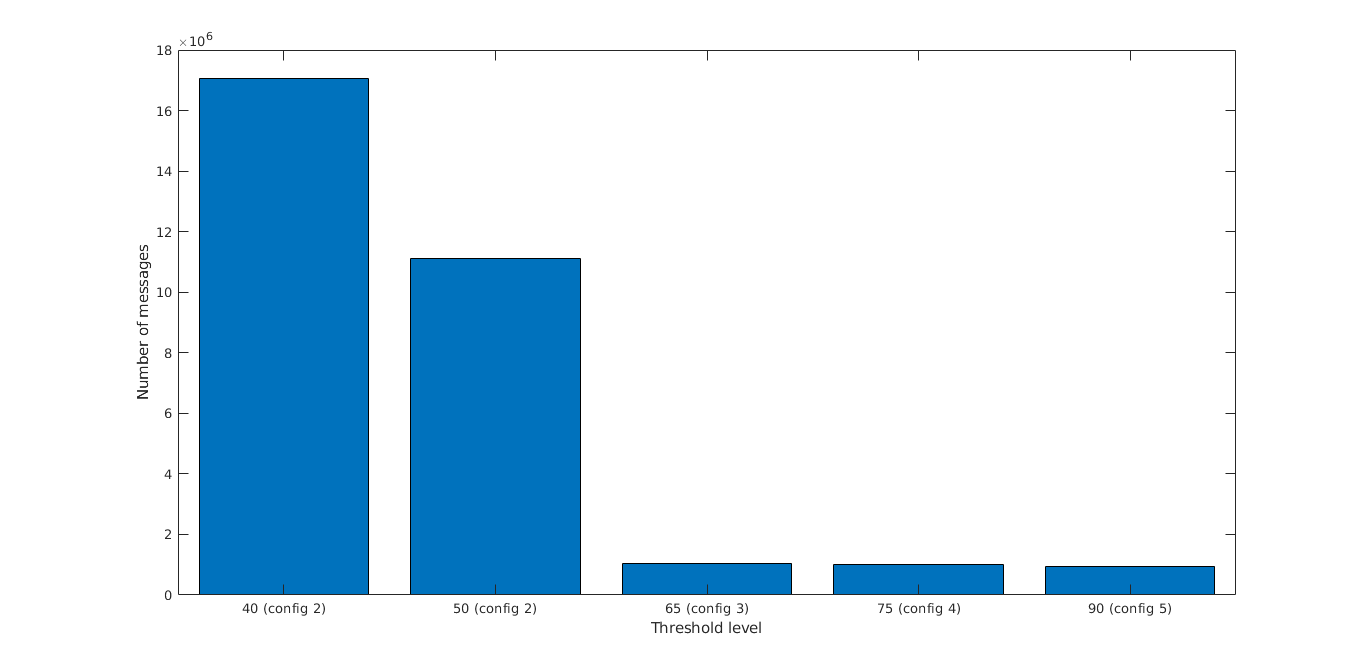
\includegraphics[width=1\linewidth]{img/threshold_messages_number.png}
	\caption{Number of messages exchanged between the agents according to the threshold level. (10 agents, View radius=40, TIME\_WAIT\_BID\_REPLY=15)}
	\label{fig:threshold-messages-number}
\end{figure}
\begin{figure}[H]
	\centering
	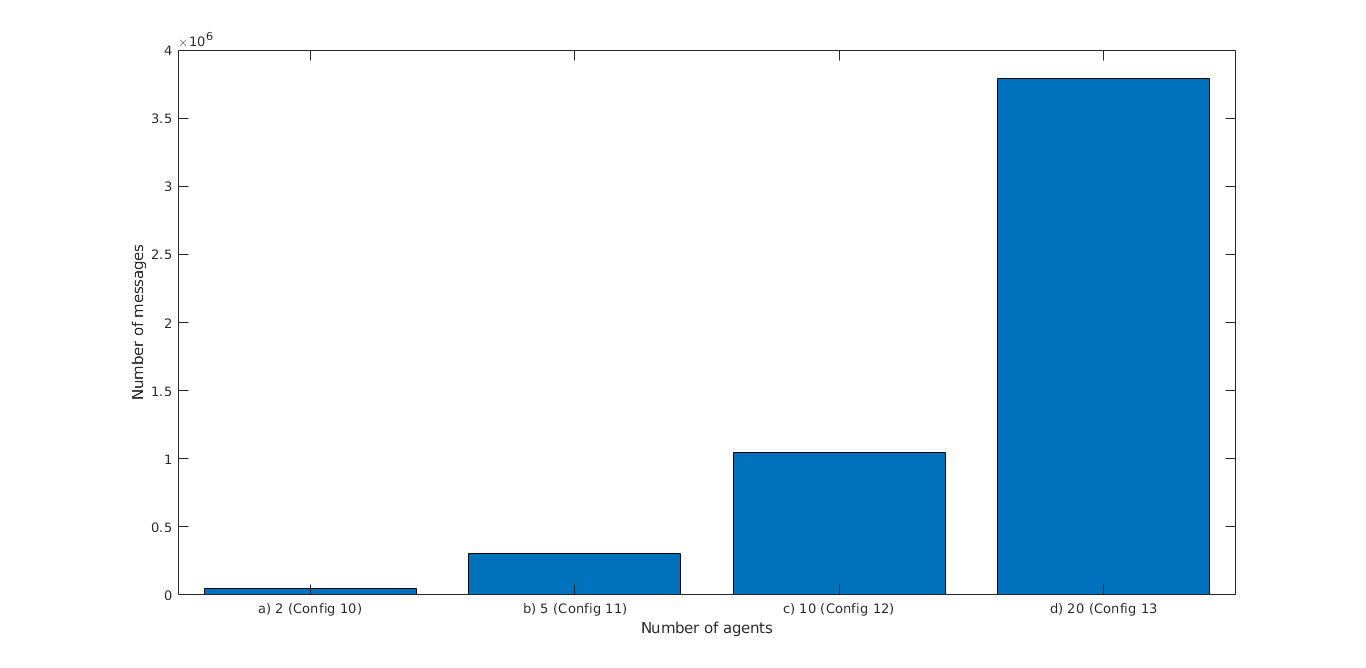
\includegraphics[width=1\linewidth]{img/agents_messages_number.png}
	\caption{Number of messages exchanged between the agents according to the number of agents. (Interest threshold=65, View radius=40, TIME\_WAIT\_BID\_REPLY=15)}
	\label{fig:agents-messages-number}
\end{figure}
\begin{figure}[H]
	\centering
	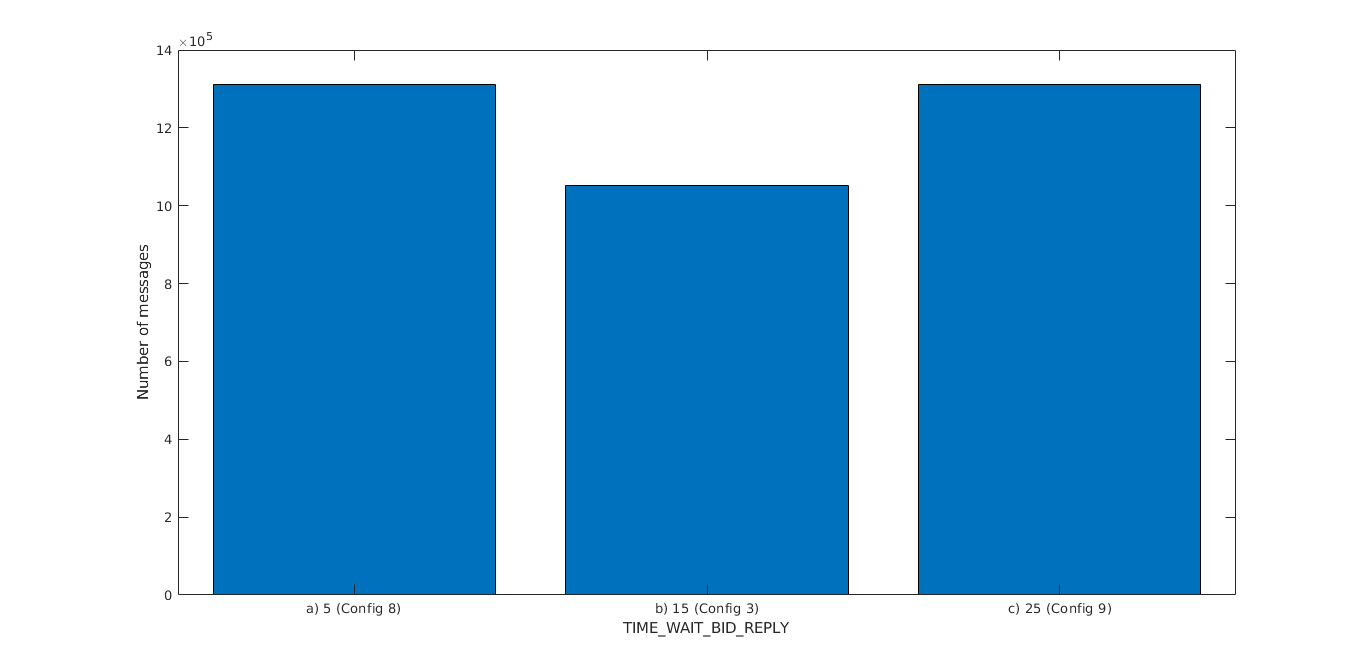
\includegraphics[width=1\linewidth]{img/time_messages_number.png}
	\caption{Number of messages exchanged between the agents according to the parameter TIME\_WAIT\_BID\_REPLY. (10 agents, Interest threshold=65, View radius=40, TIME\_WAIT\_BID\_REPLY=15)}
	\label{fig:bid-time-messages-number}
\end{figure}

Figure \ref{fig:threshold-messages-number} shows that the number of exchanged messages drastically decreases when increasing the threshold value. This is due to the fact that, when using an high threshold value, the agents tend to classify at distance the majority of the objects, reducing therefore the number of interesting objects that the agents consider worth to be visited. Consequently, the bidding algorithm is run fewer times and the number of messages exchanged is reduced. It is as well possible to note that the biggest difference in term of number of messages happens when the threshold value is raised from 50 to 65, while the number remains basically the same when increasing the threshold from 65 to 90. 

Figure \ref{fig:agents-messages-number} illustrates the trend of the messages number according to the number of agents. As expected, the number of exchanged messages grows exponentially when increasing the number of agents participating to the exploration. This is mainly due to the high overhead in term of messages brought by our bidding algorithm. This aspect has definitely to be considered when implementing such a system in a real-life scenario, since it is essential to adopt a network with performance up to the estimated number of messages that have to be carried between the agents, otherwise the network will act as a bottleneck and negatively affect the performance of the whole system.  

Finally, in figure \ref{fig:bid-time-messages-number} it is possible to note how the number of exchanged messages varies according to the time that the agents have to wait before considering themselves as the winner of an auction for a certain location, namely the value of the parameter TIME\_WAIT\_BID\_REPLY. In this case, the best results is achievable by setting the mentioned parameter to 15 seconds (which is also the value that guarantees the best performance in term of exploration time and classification error). 

\subsection{Comparison with master-slave approach used in \cite{tavaresgaspar}}
In this section we present a brief comparison between our results and the ones (concerning the structured environment) shown in \cite{tavaresgaspar}, in which a master-slave coordination approach is used in a multi-agent system to which our work is inspired to. For performing this comparison, we use analogous configurations for both the systems. In particular, we decided to use the configuration which gave us the best results in term of error and exploration time, namely Configuration 3. The configuration used for the master-slave approach system has basically the same values of our Configuration 3 and, according to \cite{tavaresgaspar}, it also corresponds to the configuration giving the best results for the structured environment. 

Having the original system implementation used in \cite{tavaresgaspar} at our disposal, we were able to directly run it in order to collect the results presented below. As we did for all the other tests, the results have been collected by running the simulation 50 times and doing an average of the obtained values. 

\begin{figure}[H]
	\centering
	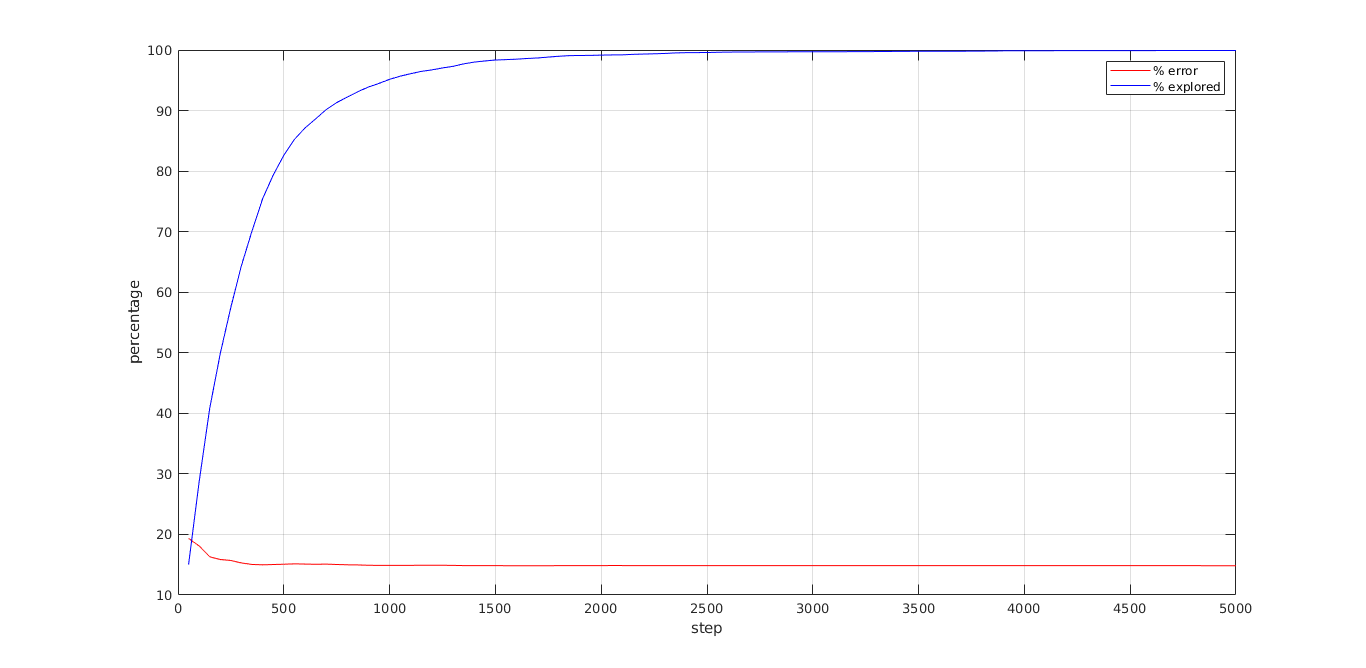
\includegraphics[width=1\linewidth]{img/exploration-original.png}
	\caption{Master-slave approach implemented in \cite{tavaresgaspar}. Structured environment, 10 Agents, Threshold=65, View radius=40}
	\label{fig:results-original}
\end{figure}
\begin{figure}[H]
	\centering
	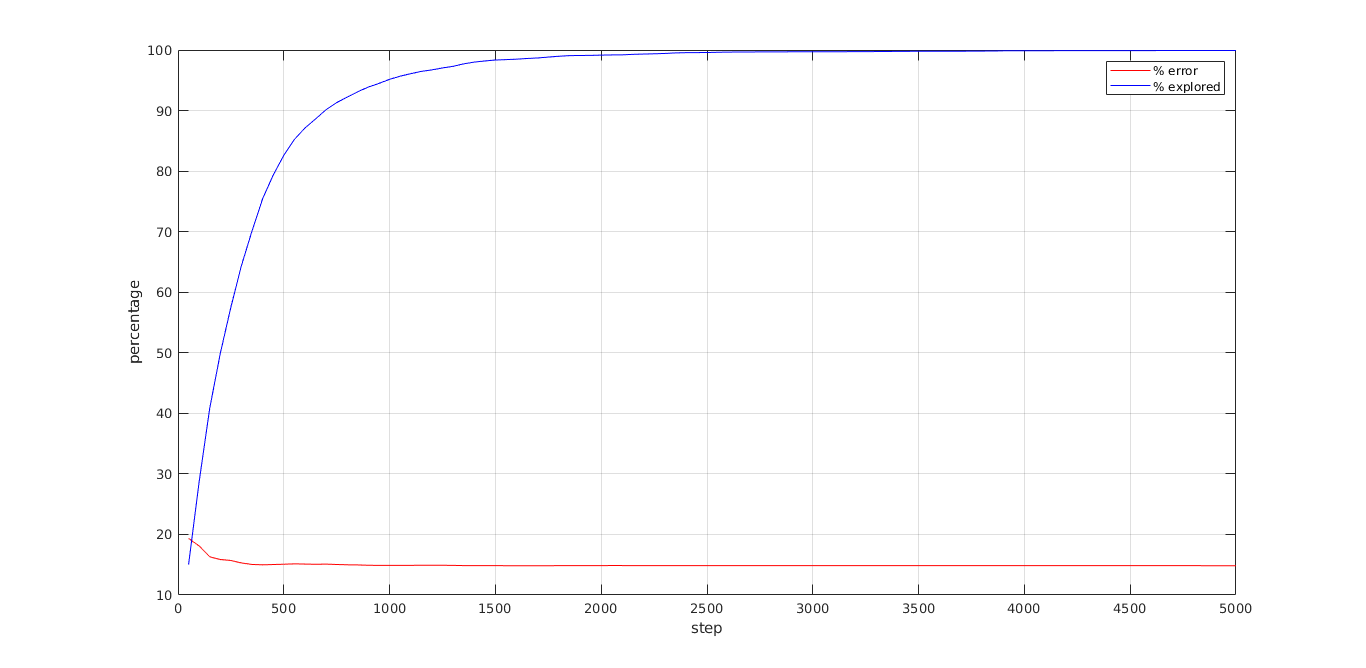
\includegraphics[width=1\linewidth]{img/exploration-original.png}
	\caption{Our peer-to-peer approach, configuration 3: structured environment, 10 Agents, Threshold=65, View radius=40}
	\label{fig:results-ours}
\end{figure}

Comparing the two plots in figure \ref{fig:results-original} and \ref{fig:results-ours}, it is possible to note how the performance of the two systems are similar. With the master slave approach, the agents are able to explore 100\% of the environment slightly quicker than with our peer-to-peer approach, while however with both the approaches 90\% of the environment gets explored after 700 simulation steps, broadly. Concerning the classification error rate, with both the approaches it stays around 15\%, even tough with the master-slave approach it is slightly smaller. 

The performance achievable with the master-slave approach are in conclusion marginally better than the one that is possible to achieve with the approach we explained in this paper. Nevertheless, as already mentioned in the introduction section, it is important to point out that our approach has the main advantage of having an higher fault-tolerance, since we do not make use of central entities from which all the agents depend on. 





\section{Conclusions}
Our approach to an exploration system is an adaptation of \cite{tavaresgaspar}, with the main difference that we decided to forgot the mediator for the agents and instead decided to implement a peer-to-peer architecture in order to remove the two single points of failure of system represented by the master entities adopted in the mentioned work, namely the \emph{Broker} and the \emph{Mapper} agents. By removing these two entities, which purpose was respectively to determine the next target of the agents and to keep a consistent map of the world known so far, we also had to adapt the process used to determine the agents targets. For this purpose, we defined and implemented a bidding algorithm that allows the agents (peers) to communicate to each other in order to determine which agent should go to visit a certain location for classifying an object that has been spotted and considered ``interesting enough''. This algorithm allowed us to merge the role of \emph{Broker} into the explorer agents themselves, which now, instead of asking to a central entity a new target location every time they reach their targets, communicate with all their other peers for determining it. The role of \emph{Mapper} has also been merged into the explorer agents: for doing so, we penalized the efficiency of the system and we made the explorers broadcast to all their peers every single new information they get about the environment they are exploring. 

The results we collected from the simulations are very similar to the ones obtained by \cite{tavaresgaspar}, even though our approach brings a considerable increase of the number of messages exchanged between the agents. On the other hand, our system is not affected by the possibility that the failure of a single agent can compromise the working of the whole system, and therefore it can be considered more robust. We believe that this feature is particularly useful, especially in those environments where agents have no previous knowledge of their surroundings and where there is no way to access them for performing a repair, like, for instance, remote planets in the space exploration context. In such a scenario, if one of the master agents stops working, there is no way for the other agents to continue their exploration, while our approach would make up for such a flaw. 

However, the price we had to pay for having a fault-tolerance improvement is represented by the remarkable number of messages exchanged between the agents. Indeed, the bidding algorithm we designed requires an heavy and steady communication between the agents, which also have to constantly broadcast to their peers every new information they get, so that they can share they knowledge and keep their maps of the environment always updated. This involves that, when implementing a real system using such approach, more attention has to be given to the design of the network connecting the agents. The network, in fact, has to be performing enough for delivering a substantial amount of messages (the number of messages, as shown in section \ref{sec:resuslts}, grows exponentially with the number of agents involved) with an as much as possible reduced delay, in order to limit any eventual inconsistency between the maps of the single agents and to avoid it to become a bottleneck for the system. Concerning this last aspect, using the approach adopted in \cite{tavaresgaspar}, both the Mapper and the Broker entities represented a potential bottleneck for the system, consequently, we can as well consider that with our approach the number of potential bottlenecks has been reduced to one (e.g. the network). 

In conclusion, we believe that the approach we presented in this paper can be a valid alternative to the one shown in \cite{tavaresgaspar}. From the collected results, it is possible to assert that the performance achievable with the two approaches, in term of exploration time and classification error, are decidedly similar. Even though the proposed approach has the drawback of having lower efficiency, we believe this to be a marginal aspect when compared to the fault-tolerance improvement that it gives to the system, considering that fault-tolerance is often critical in unknown environments exploration. Furthermore, it is not excluded that our approach can be improved in order to reduce the communication overhead between the agents: in this way, the system we implemented would represent a preferable alternative to the one shown in \cite{tavaresgaspar}.

%  *********** CITE THIS IN FUTURE WORK SECTION *************************
%However, our system is not without flaws: should there not be any interesting locations for the agents to explore then they will wander around the environment randomly while another attitude from the agents would perhaps yield better results. That could be a new aspect to implement for the future. Currently, as the system stands, it presents satisfactory results. As it stands, we can state that for unknown environments, our system is a reliable approach.    

\section{Future work}
From the results we collected, it is easy to notice the the   main limit of our system, represented by the high communication overhead it carries. In this way, as already mentioned, the system could be improved in order to address this lack of efficiency, adopting for instance a distributed algorithm for efficiently merging the maps of the single agents, without making them broadcast every single new information they get. This would definitely reduce the overall number of message exchanged. 

Another aspect that could be improved is the behaviour of the agents when they do not have any more interesting points to visit (potential targets), even though the environment has not been completely explored yet. In this situation, the agents decide their new targets in a random way until the environment is fully explored. An alternative behaviour for the agents when this situation occurs would be worth to be defined. 

Finally, as already proposed in \cite{tavaresgaspar}, a self-policing behavior of the agents could be developed, by making them check periodically for classification errors and adapting the system accordingly, for instance by resetting the prototypes or updating the respective weights. 


\addtolength{\textheight}{-12cm}   % This command serves to balance the column lengths
                                  % on the last page of the document manually. It shortens
                                  % the textheight of the last page by a suitable amount.
                                  % This command does not take effect until the next page
                                  % so it should come on the page before the last. Make
                                  % sure that you do not shorten the textheight too much.

%%%%%%%%%%%%%%%%%%%%%%%%%%%%%%%%%%%%%%%%%%%%%%%%%%%%%%%%%%%%%%%%%%%%%%%%%%%%%%%%



%%%%%%%%%%%%%%%%%%%%%%%%%%%%%%%%%%%%%%%%%%%%%%%%%%%%%%%%%%%%%%%%%%%%%%%%%%%%%%%%



%%%%%%%%%%%%%%%%%%%%%%%%%%%%%%%%%%%%%%%%%%%%%%%%%%%%%%%%%%%%%%%%%%%%%%%%%%%%%%%%
\section*{APPENDIX}
In this appendix we provide a brief tutorial for downloading and executing the system described in this paper. The source code is publicly available on \href{https://gitlab.com/Telemaco019/ai-exploration-project}{this Git repository} and all the relevant Java classes are included in the package \emph{sim.app.exploration}. For simplicity, it is assumed that the IDE being used is IntellijIDEA \cite{intellij} (the step are similar for any other IDE). 
\begin{enumerate}
    \item Create a new ``Project from version control''
    \item Select Git and specify the URL of the project repository 
    \item Add to the project the dependencies to all the libraries included in the folder ``resources'': 
    \begin{enumerate}
        \item ``File $\rightarrow$ Project Structure $\rightarrow$ Libraries''
        \item ``Add new library from Java''
        \item Select all the libraries included in the folder ``resources''
        \item Confirm
    \end{enumerate}
    \item If it has not been done automatically, set the SDK for the project. Version 1.8 or higher is required.
    \begin{enumerate}
        \item ``File $\rightarrow$ Project Structure $\rightarrow$ Project''
        \item Select the SDK from the menu
        \item Set ``Project language level'' to ``8 - Lambdas, type annotations etc.''
    \end{enumerate}
    \item Mark the folder ``mason'' as source folder: 
    \begin{enumerate}
        \item ``File $\rightarrow$ Project Structure $\rightarrow$ Modules''
        \item Click on the folder ``mason'' and then on ``Mark as: sources''
        \item Confirm
    \end{enumerate}
    \item Create a new run configuration:
    \begin{enumerate}
        \item Select ``Add configuration\dots $\rightarrow$ Application''
        \item For running the program with the GUI, select as main class ``Viewer'', which is included in the package \emph{sim.app.exploration.core}. For running instead the program a certain number of times without the GUI in order to get the data for the plots, select as main class ``Simulator'', which can be as well found in the package \emph{sim.app.exploration.core}
    \end{enumerate}
    \item Run the previously created configuration
\end{enumerate}

After running the program, the the statistics of the execution are saved in a .csv file in the folder ``stats''. This folder also contains a Matlab script for plotting the results (the script read all the .csv files included in the stats folder, compute an average of the values they contains and plot it). 

\section*{ACKNOWLEDGMENT}


\printbibliography

\end{document}
